\documentclass{aiaa-tc}
\usepackage{amsmath,epstopdf}
\usepackage{subfigure,morefloats}
\usepackage{caption,multirow}
\usepackage{subfigmat}
\usepackage{caption}
\usepackage{bbding}

\newcommand{\psibold}{\mbox{\boldmath$\psi$}}
\newcommand{\nablabold}{\mbox{\boldmath$\nabla$}}
\newcommand{\sigmabold}{\mbox{\boldmath$\sigma$}}
\newcommand{\Omegabold}{\mbox{\boldmath$\Omega$}}
\newcommand{\Gammabold}{\mbox{\boldmath$\Gamma$}}
\newcommand{\degr}{ ^{\circ}}
\renewcommand{\l}{\left}
\renewcommand{\r}{\right}

%List of authors:
%Manuel R. L\'opez-Morales
%Abhishek Sheshadri
%Kartikey Asthana
%Jacob Crabill
%Thomas Economon
%David Manosalvas
%Joshua Romero
%Jerry Watkins
%David Williams
%Dr. Francisco Palacios
%Prof. Antony Jameson

\title{Verification and Validation of HiFiLES: a High-Order LES unstructured solver on multi-GPU platforms}

 \author{Manuel R. L\'opez-Morales
         \thanks{Ph.D. Candidate, Department of Aeronautics and Astronautics, Stanford University, AIAA Student Member; mlopez14@stanford.edu},
            Jonathan Bull\thanks{Postdoctoral Scholar, Department of Aeronautics and Astronautics, Stanford University, AIAA Member},
            Jacob Crabill,\thanks{Ph.D. Candidates (authors in alphabetical order), Department of Aeronautics and Astronautics, AIAA Student Members},\\
            Thomas D. Economon\footnotemark[3],
            David Manosalvas\footnotemark[3],\\
            Joshua Romero\footnotemark[3],
            Abhishek Sheshadri \footnotemark[3],
            Jerry E. Watkins II\footnotemark[3],
            David Williams\thanks{CFD Engineer, Flight Sciences Division, Boeing Commercial Airplanes, AIAA Member},\\
            Francisco Palacios\thanks{Engineering Research Associate, Department of Aeronautics and Astronautics, AIAA Senior Member}, and
            Antony Jameson\thanks{Thomas V. Jones Professor of Engineering, Department of Aeronautics and Astronautics, Stanford University, AIAA Fellow} \\
           \normalsize\itshape
         Department of Aeronautics and Astronautics, Stanford University, Stanford, CA, 94305 \vspace{0.1in}
         }


\begin{document}

\maketitle

% !TEX root = ./main.tex

\begin{abstract}
The goal of this paper is to show a detailed Verification and Validation of HiFiLES: a high-order Navier-Stokes solver developed at the Aerospace Computing Laboratory (ACL) at Stanford University. HiFiLES has been built on top of SD++ (Castonguay et al.) and achieves high-order spatial discretization with the Energy-Stable Flux Reconstruction (ESFR) scheme in unstructured grids (two and three dimensions). The high parallelizability of this scheme motivates the optimization of the solver’s ability to run in a multi-GPU (Graphical Processing Unit) environment.
We intend this paper to be the main reference for HiFiLES and serve as a sort of manual for researchers and engineers that would like to develop or implement high-order numerical schemes based on an Energy-Stable Flux Reconstruction (ESFR) scheme.
%Verification and validation studies performed on the Navier-Stokes (NS) solver HiFiLES are presented. \\HiFiLES achieves high-order spatial discretization with the Energy-Stable Flux Reconstruction (ESFR) scheme in unstructured grids in two and three dimensions. The high parallelizability of this scheme motivates the optimization of the solver's ability to run in a multi-GPU (Graphical Processing Unit) environment with the ability to run in a CPU (Central Processing Unit) cluster. In addition, to exploit such parallelizability, implicit time advancement is realized with dual time-stepping and p-multigrid acceleration. HiFiLES includes a suite of Sub-Grid Scale (SGS) models and filters in order to perform Large Eddy Simulations (LES). To ensure the implementation of the aforementioned features in HiFiLES is correct, the following verification tests were performed: check of spatial and temporal order of accuracy using the Method of Manufactured Solutions in 2D and 3D for viscous and inviscid flows, characterization of stable time-step limits, assessment of computational cost per degree of freedom for a given error tolerance, and measurement of weak and strong scalability in GPUs and CPUs. The simulations of complex flows were validated against experimental or Direct Numerical Simulation (DNS) results for the following cases: flow around a circular cylinder, SD7003 wing-section and airfoil at 4$\degr$ angle of attack, DNS of the Taylor-Green Vortex, and DNS and LES of Decaying Homogeneous Turbulence.
\end{abstract}

%% !TEX root = ./main.tex

\section*{Nomenclature}

 \begin{tabbing}
  XXXXXXXXXXX \= \kill % first line sets tab stop

$\Omega$ \> Simulation domain \\
$\Omega_s$ \> Reference element domain \\
$\Gamma$ \> Element mapping: physical to reference domain \\
$\lambda$ \> Viscosity of medium \\
$\eta^e$ \> Bassi Rebay weighting constant \\

$c$ \> Correction function parameter \\
$f, \hat{f}^{\delta} $ \> Inviscid flux, untransformed and transformed \\
%$\hat{f}^{\delta D}$\hat{f}^{\delta I}, \hat{f}^{\delta C} $ \> Inviscid flux, discontinuous, interface, correction \\

$f_v, \hat{f_v}^{\delta} $ \> Viscous flux, untransformed and transformed \\
%$\hat{f_v}^{\delta D}, \hat{f_v}^{\delta I}, \hat{f_v}^{\delta C} $ \> Viscous flux, discontinuous, interface, correction \\

$g, g_L, g_R$ \> Correction functions, generic, left and right interfaces \\

$J$ \> Element jacobian \\

$k$ \> Degree of discontinuous solution basis \\
$L_k$ \> Legendre polynomial degree k \\
$l_k$ \> Lagrange polynomial degree k \\

$r$ \> Coordinate in reference domain \\
$r_e$ \> Bassi Rebay lifting operator \\
$t$ \> Time based on simulation units \\
$u, \hat{u}^{\delta} $ \> Solution, untransformed and transformed \\
%$\hat{u}^{\delta D}, \hat{u}^{\delta I}, \hat{u}^{\delta C} $ \> Solution flux, discontinuous, interface, correction \\
$x$ \> Coordinate in physical domain \\

 \end{tabbing}

% !TEX root = ./main.tex

\section{Introduction}

Over the last 20 years, much fundamental work has been done in developing high-order numerical methods for Computational Fluid Dynamics. The need to improve and simplify these methods has attracted the interest of the applied mathematics and the engineering communities. Now these methods are beginning to prove themselves sufficiently robust, accurate, and efficient for use in real-world applications.

However, low-order numerical methods are still the standard in the aeronautical industry. There has been a sustained scientific and economical investment to develop this successful and robust technology for a long time. Currently, a state-of-the-art 2nd-order Finite Volume computational tool performs adequately well in a broad range of aeronautical engineering applications. For that reason, the introduction of brand-new high-order numerical schemes in the aeronautical industry is challenging, particularly in areas where the low-order numerical methods already provide the required robustness and accuracy (keeping in mind the limitations of the current turbulence model technology).

Thanks to new and emerging aircraft roles (very small or very big concepts, very high or very low altitude, quiet vehicles, low fuel consumption, etc.), revolutionary aircraft design concepts will appear in the near future and the need for high-fidelity simulation techniques to predict their performance is growing rapidly. Undoubtedly, high-order numerical methods are starting to find their place in the aeronautical industry. 

Unsteady simulation, flapping wings, wake capturing, noise prediction, and Large Eddy Simulation (LES) are just a few examples of computations that require high-order numerical methods. In particular, high-order methods have a significant edge in applications that require accurate resolution of the smallest scales of the flow. Such situations include the generation and propagation of acoustic noise from the airframe, or at the limits of the flight envelope where unsteady vortex-dominated flows have a significant effect on the aircraft's performance. Utilizing a high-order representation enables the smallest scales to be represented with a greater degree of accuracy than standard second-order methods. Furthermore, high-order methods are inherently less dissipative, resulting in less unwanted interference with the correct development of the turbulent energy cascade. This factor makes the combination of high-order numerics with LES modeling very powerful, with the potential to significantly improve upon the accuracy and computational cost of the standard approach of LES with second-order methods.

Finally, the amount of computing effort to achieve a small error tolerance can be much smaller with high-order than second-order methods. Even real time simulations (one second of computational time, one second of real flight), could benefit from high-order algorithms which count on a more intensive inner element computation (ideal for vector machines and new computational platforms like GPUs, FPGAs, coprocessors, etc).

But, before claiming the future success of the high-order numerical methods in the industry, two main difficulties should be overcome: a) high-order numerical schemes must be as robust as state-of-the-art low-order numerical methods, b) the existing level of Verification and Validation (V\&V) in high-order CFD codes should be similar to the typical level of their low-order counterparts.

During the last decade, the Aerospace Computing Laboratory (ACL) of the Department of Aeronautics and Astronautics at Stanford University has developed a series of high-order numerical schemes and computational tools, contributing massively to the demonstration of the viability of this technique. In this paper, a code called HiFiLES developed at ACL and built on top of SD++ (Castonguay et al.\cite{castonguay2011}) is described in detail with a particular emphasis on robustness in a range of applications and an industrial-like level of V\&V. %HiFiLES takes advantage of the synergies between applied mathematics, aerospace engineering, and computer science to achieve the ultimate goal of developing an advanced high-fidelity simulation environment.

Apart from the original characteristics of the SD++ code (described in Castonguay et al.\cite{castonguay2011}), HiFiLES includes some important physical models and computational methods such as: Large Eddy Simulation (LES) using explicit filters and advanced subgrid-scale (SGS) models, high-order stabilization techniques, shock detection and capturing for compressible flow calculations, convergence acceleration methodologies like p-multigrid, and local and dual time stepping. Some of these techniques will be described in this or related papers.

During the development of this software several key decisions have been taken to guarantee a flexible and lasting infrastructure for industrial Computational Fluid Dynamics simulations:
\begin{itemize}
\item The selection of the Energy-Stable Flux Reconstruction (ESFR) scheme on unstructured grids. The flexibility of this method has been critical to guarantee a correct solution independently of the particular physical characteristics of the problem.
\item High performance, materialized in a multi-GPU implementation which takes advantage of the ease of parallelization afforded by discontinuous solution representation. Furthermore, HiFiLES aims to guarantee compatibility with future vector machines and revolutionary hardware technologies.
\item Code portability by using ANSI C++ and relying on widely-available, and well-supported mathematical libraries like Blas, LAPACK, CuBLAS and ParMetis.
\item Object oriented structure to boost the re-usability and encapsulation of the code. %This abstraction enables modifications without incorrectly affecting other portions of the code. Although some level of performance is traded for re-usability and encapsulation, the loss in performance is minor.
\end{itemize}

As mentioned before, the mathematical basis and computational implementation of HiFiLES were described in Castonguay et al.\cite{castonguay2011}. For that reason, the goal of this paper is to illustrate the level of robustness of HiFiLES in interesting problems, via a Verification and Validation study which is fundamental to increase the credibility of this technology in a competitive industrial framework.

In particular, to ensure that the implementation of the aforementioned features in HiFiLES is correct, the following verification tests are shown: checks of spatial and temporal order of accuracy using the Method of Manufactured Solutions (MMS) in 2D and 3D for viscous and inviscid flows and characterization of stable time-step limits. After the Verification, a detailed Validation of the code is presented to illustrate that the solutions provided by HiFiLES are an accurate representation of the real world. Simulations of complex flows are validated against experimental or Direct Numerical Simulation (DNS) results for the following cases: laminar flat-plane, flow around a circular cylinder, SD7003 wing-section and airfoil at 4$\degr$ angle of attack, the Taylor-Green Vortex and LES of a square cylinder.

The organization of this paper is as follows. Section \ref{sec:govEq} provides a description of the governing equations. Section \ref{sec:numerics} describes the mathematical numerical algorithms implemented in the code (with a particular emphasis in convergence acceleration techniques and stability). \ref{sec:verification} describes the Verification and Validation of HiFiLES, and finally, the conclusions are summarized in section \ref{sec:conclusion}

Finally, it is our intent for this paper to be the main reference for work that uses or enhances the capabilities of HiFiLES, and for it to serve as a sort of reference for researchers and engineers that would like to develop or implement High-order numerical schemes based on an Energy-Stable Flux Reconstruction (ESFR) scheme.

% !TEX root = ./main.tex

\section{Governing Equations}
\label{sec:govEq}
\subsection{Navier Stokes (NS) Equations}
The main purpose of HiFiLES is to perform High-Fidelity Large-Eddy Simulations --hence the name. The form of the NS Equations most useful for understanding how the FR methodology can be used to solve them is the following
\begin{equation}
\frac{\partial U}{\partial t} +  \nabla \cdot {\bf F} = 0
\end{equation}

where ${\bf F} = (F,G,H) = (F_I,G_I,H_I) - (F_V,G_V,H_V)$ and
\begin{equation}
U = \l(
\begin{tabular}{c}
$\rho$\\
$\rho u$\\
$\rho v$\\
$\rho w$\\
$\rho e$
\end{tabular}
\r) \;\; 
F_I = \l(
\begin{tabular}{c}
$\rho u$\\
$\rho u^2 + p$\\
$\rho uv$\\
$\rho uw$\\
$\rho ue + p$
\end{tabular}
\r) \;\; 
G_I = \l(
\begin{tabular}{c}
$\rho v$\\
$\rho vu$\\
$\rho v^2 + p$\\
$\rho vw$\\
$\rho ve+p$
\end{tabular}
\r) \;\; 
H_I = \l(
\begin{tabular}{c}
$\rho w$\\
$\rho wu$\\
$\rho wv$\\
$\rho w^2 + p$\\
$\rho we + p$
\end{tabular}
\r) \;\; 
\end{equation}
\begin{equation}
F_V = \l(
\begin{tabular}{c}
$0$\\
$\sigma_{xx}$\\
$\sigma_{xy}$\\
$\sigma_{xz}$\\
$u_i\sigma_{ix}-q_x$
\end{tabular}
\r) \;\; 
G_V = \l(
\begin{tabular}{c}
$0$\\
$\sigma_{yx}$\\
$\sigma_{yy}$\\
$\sigma_{yz}$\\
$u_i\sigma_{iy}-q_y$
\end{tabular}
\r) \;\; 
F_V = \l(
\begin{tabular}{c}
$0$\\
$\sigma_{zx}$\\
$\sigma_{zy}$\\
$\sigma_{zz}$\\
$u_i\sigma_{iz}-q_z$
\end{tabular}
\r) \;\; 
\end{equation}

As usual, $\rho$ is density, $u$, $v$, $w$ are the velocity components in the $x, y, z$ directions, respectively, and $e$ is total energy per unit mass. In HiFiLES, the pressure is determined from the ideal gas equation of state
\begin{equation}
p = (\gamma - 1)\rho\l(e - \frac{1}{2}\l(u^2 + v^2 + w^2\r)\r)
\end{equation}
the viscous stresses are those of a Newtonian fluid
\begin{equation}\label{sigma}
\sigma_{ij} = \mu\l( \frac{\partial u_i}{\partial x_j}
+ \frac{\partial u_j}{\partial x_i} \r)
- \frac{2}{3}\mu \delta_{ij}\frac{\partial u_k}{\partial x_k}
\end{equation}
and the heat fluxes are defined as
\begin{equation}
q_i = -k \frac{\partial T}{\partial x_i}
\end{equation}
where
\begin{equation}
k = \frac{C_p \mu}{\text{Pr}} , \;\; T = \frac{p}{R \rho}
\end{equation}

Pr is the Prandtl number, $C_p$ is the specific heat at constant pressure and $R$ is the gas constant. In the case of air, $\gamma = 1.4$ and Pr $= 0.72$. The dynamic viscosity $\mu$ in HiFiLES can be a constant or a function of temperature using Sutherland's law.


\subsection{Reynolds Averaged Navier-Stokes (RANS) equations}
The compressible NS equations can be used to solve a variety of different flow physics problems but for turbulent flows, direct numerical simulation using these equations can become excessively expensive. For engineering applications, it is customary to perform a Favre averaging procedure to the NS equations to solve a turbulent mean quantity. This leads to a variety of terms which must be modeled in order to provide closure to the resulting RANS equations \cite{wilcox1998turbulence,oliver2008high}. The conservative form of the equations is very similar to the NS equations with an added source term:
\begin{align}
	\frac{\partial \boldsymbol{U}}{\partial t} + \nabla \cdot \boldsymbol{F} = \boldsymbol{Q}
\end{align}
The conservative variables are now averaged quantities and the RANS equations must now be solved with an appropriate turbulence model.


% !TEX root = ./main.tex

\section{Numerical Methods}
\label{sec:numerics}

In this section the main numerical techniques implemented in HiFiLES will be described. We will emphasize the critical role of the selected numerical discretization (Flux Reconstruction Method), and it capability to solve CFD problems using unstructured meshes. 

\subsection{Flux Reconstruction Method}

What follows is an overview of the flux reconstruction (FR) framework. We start the discussion with the solution of the advection-diffusion equation in one dimension using the FR approach to illustrate the method. We then proceed to briefly explain how conservation equations can be solved in multiple dimensions. The Navier-Stokes equations are a set of coupled conservation equations in multiple dimensions, so the extension of the FR methodology to them is straightforward. The detailed description of the algorithm used in HiFiLES is given by Castonguay et al. \cite{castonguay2011}.

\subsubsection{Solution of the Advection Equation in One Dimension using the FR Approach}

Consider the one-dimensional conservation law
\begin{equation}
\label{eq:cons}
\frac{\partial u}{\partial t} + \frac{\partial f}{\partial x} = 0
\end{equation}

in domain $\Omega$, where $x$ is the spatial coordinate, $t$ is time, $u$ --the \emph{solution}-- is a scalar function of $x$ and $t$, and $f$ --the \emph{flux}-- is a scalar function of $u$. Note that by letting $f = f(u,\frac{\partial u}{\partial x})$, Equation~\ref{eq:cons} becomes a model of the Navier-Stokes equations.

Let us partition the domain $\Omega = [x_1,x_{N+1})$ into $N$ non-overlapping elements with 
interfaces at $x_1<x_2<...<x_{N+1}$. Then,
\begin{equation}
\Omega = \bigcup^N_{n=1} \Omega_n
\end{equation}
and $\Omega_n = [x_n,x_{n+1})$ for $n = 1,...,N$. To simplify the implementation, let us map each of the physical elements $\Omega_n$ to a standard element $\Omega_s=[-1,1)$ with the function $\Theta_n(\xi)$, where
\begin{equation}
x = \Theta_n(\xi) = \l( \frac{1-\xi}{2} \r) x_n + \l(\frac{1+\xi}{2}\r) x_{n+1} 
\end{equation}

With this mapping, the evolution of $u$ within each $\Omega_n$ can be determined with the following 
transformed conservation equation
\begin{equation}
\frac{\partial \hat{u}}{\partial t} + \frac{1}{J_n}\frac{\partial \hat{f}}{\partial \xi} = 0
\end{equation}
where
\begin{equation}
\hat{u} = u(\Theta_n(\xi),t) \text{ in } \Omega_n
\end{equation}
\begin{equation}
\hat{f} = f(\Theta_n(\xi),t) \text{ in } \Omega_n
\end{equation}
\begin{equation}
J_n = \frac{\partial x}{\partial \xi} \bigg|_{\Omega_n}
\end{equation}

Now, we introduce polynomials of degree $p$, $\hat{u}^\delta$ and $\hat{f}^\delta$, to approximate the exact values $\hat{u},\hat{f}$, respectively. We can write these polynomials as
\begin{equation}
\hat{u}^\delta = \sum_{i=1}^{N_s} \hat{u}_i^\delta l_i(\xi)
\end{equation}
\begin{equation}
\hat{f}^\delta = \sum_{i=1}^{N_s} \hat{f}_i^\delta l_i(\xi)
\end{equation}
where $N_s$ is the number of solution points, $\hat{u}_i^\delta$ is the current value of the 
solution approximation function at the $i^\text{th}$ \emph{solution point} in the reference element, 
$\hat{f}_i^\delta$ is the current value of the flux approximation function at the $i^\text{th}$ 
\emph{flux point} in the reference element, $l_i$ is the Lagrange polynomial equal to $1$ at the 
$i^\text{th}$ solution point and $0$ at the others, and $\delta$ denotes that the function is an 
approximation.

Note that the piecewise polynomials might not be continuous (or $C^0$) across the interfaces. In the 
Flux Reconstruction approach, the flux used in the time advancement of the solution is made $C^0$ 
by introducing flux correction functions.

This can be achieved by finding interface solution values at each element boundary and then correcting the 
solution. Let $\hat{u}_L^{\delta I}$ and $\hat{u}_R^{\delta I}$ be the interface solution values at left and right 
boundaries of some element, respectively. $\hat{u}_L^{\delta I}$ and $\hat{u}_R^{\delta I}$ can be found with a Riemann solver for Discontinuous-Galerkin (DG) methods\cite{hesthaven2007}. Then, select solution correction functions $g_L$ and 
$g_R$ such 
that
\begin{equation}\label{eq:condition}
g_L(-1) = 1 \;,\; g_L(1) = 0
\end{equation}
\begin{equation}
g_R(-1) = 0 \;,\; g_R(1) = 1
\end{equation}
and let
\begin{equation}
\hat{u}^C = \hat{u}^\delta + (\hat{u}^{\delta I}_L - \hat{u}^\delta_L) g_L + (\hat{u}^{\delta I}_R 
- \hat{u}^\delta_R) g_R
\end{equation}
where superscript $C$ denotes the function is corrected, and $\hat{u}^\delta_L$, $\hat{u}^\delta_R$ 
represent the solution approximation evaluated at the left and right boundaries.

Using the values of $\hat{u}^\delta_i$ and $\frac{\partial \hat{u}^C}{\partial \xi}|_{\xi_i}$ we then find 
$$\hat{f}_i^\delta = \hat{f}\l(\hat{u}^\delta_i,\frac{1}{J_n}\frac{\partial \hat{u}^C}{\partial \xi}\bigg|_{\xi_i}\r) \;\; \text{in element } \Omega_n$$
We can proceed in a similar fashion to correct the flux to obtain
\begin{equation}
\hat{f}^C = \hat{f}^\delta + (\hat{f}^{\delta I}_L - \hat{f}^\delta_L) h_L + (\hat{f}^{\delta I}_R 
- \hat{f}^\delta_R) h_R
\end{equation}
where $h_R$ and $h_L$ are right and left flux correction functions satisfying the same boundary 
conditions as $g_R$ and $g_L$, respectively, and $\hat{f}_L^{\delta I}$ and $\hat{f}_R^{\delta I}$ are the interface fluxes found via a Riemann solver. Note that if the flux corresponds to linear advection, correcting the solution and correcting the flux are equivalent steps.

The solution can then be advanced at each solution point. In semi-discrete form, this is
\begin{equation}\label{eq:semidiscrete}
\frac{d \hat{u}_i^\delta}{d t} = - \frac{\partial \hat{f}^c}{\partial \xi}(\xi_i)
\end{equation}

The FR scheme can be made provably stable for the linear advection-diffusion equation by selecting special types of correction functions\cite{castonguay2013}. In general, these correction functions are polynomials of degree $p+1$ so both sides in Equation~\eqref{eq:semidiscrete} are quantities related to polynomials of order $p$ --for consistency\cite{huynh2007}.

Vincent et al. \cite{vincent2011new} have shown that in the case of the 1-dimensional, linear advection equation, the Flux Reconstruction approach can be proven to be stable for a specific family of correction functions parameterized by a scalar called $c$. In addition, they showed that by selecting specific values of $c$ it is possible to recover a particular nodal Discontinuous Galerkin (DG) and Spectral Difference (SD) methods plus a FR scheme that was previously found to be stable by Huynh\cite{huynh2007flux}.

\subsection{Extension to Multiple Dimensions}

Extension to multiple dimensions requires formulating multi-dimensional interpolation functions and correction functions that satisfy boundary conditions equivalent to those in Equation~\eqref{eq:condition} for each type of element.

Interpolation bases for quadrilaterals and hexahedra can be obtained via tensor products of the 1-dimensional interpolation basis. In HiFiLES, we discretize the solution in 3-dimensions in the following way
\begin{equation}
{\bf \hat{u}}^\delta(\xi,\eta,\zeta) = \sum_{i=1}^{p+1} \sum_{j=1}^{p+1} \sum_{k=1}^{p+1}
{\bf \hat{u}}^\delta_{i,j,k} l_i(\xi) l_j(\eta) l_k(\zeta)
\end{equation}
where $i$, $j$, $k$ index the solution points along the $\xi, \eta, \zeta$ directions, respectively. The flux is discretized similarly.

The interpolation basis for triangles are described in detail by Castonguay et al. \cite{castonguay2012new} and Williams et al. \cite{williams2013tri}. The formulation for tetrahedra is detailed by Williams et al. \cite{williams2013tet}. The extension of interpolation polynomials to prisms is obtained via tensor products of the 1-dimensional basis with the triangular basis\cite{castonguay2011}. 

In general, the boundary conditions for the correction functions in multiple dimensions can be formulated as
\begin{equation}\label{eq:genConstraint}
{\bf h}_i( \vec{\xi}_j)\cdot {\bf n}_j = \delta_{ij}
\end{equation}
where ${\bf h}_i$ is the vector of correction functions associated with interface point $i$, $\vec{\xi}_j$ is the location vector of the $j^\text{th}$ interface point, ${\bf n}_j$ is the outward unit normal at interface point $j$, and $\delta_{ij}$ is the Kronecker delta. Interface points are located on the boundary of an element.

One of the challenges in the FR approach is finding correction functions that not only satisfy Equation~\eqref{eq:genConstraint} but also guarantee stability in the linear advection-diffusion case. Correction functions that guarantee such stability exist for 1-dimensional segments\cite{vincent2011new}, triangles\cite{castonguay2012new,williams2013tri}, and tetrahedra\cite{williams2013tet}. FR schemes with these correction functions comprise the ESFR family of schemes.

Although formal proofs of stability for the linear advection equation do not exist yet for quadrilaterals, hexahedra, and prisms, it has been observed that the tensor products of provably stable correction functions used in these elements maintain stability. In addition, as of now HiFiLES does not have an implementation for pyramidal elements, mostly because of the challenges involved in finding the respective correction functions that guarantee stability. Nevertheless, a suggested approach to find such correction functions has been presented by Jameson\cite{jameson2011advances}.

In terms of time integration, HiFiLES uses an explicit Adaptive Runge-Kutta 45 (RK45) Method and local or global time stepping. Currently, a polynomial multigrid to improve the code convergence is being validated.

\subsection{Shock Capturing and Stabilization Models}

We use the method of concentration described in \cite{abhishekshockcapture} for detecting shocks on meshes with quadrilateral elements. We are still in the process of extending the method of concentration to triangles and are currently using Persson and Peraire's method \cite{Persson06} \cite{Persson13} for the same. We have explored both selective addition of artificial viscosity as well as modal order reduction for capturing the detected shocks effectively. Persson and Peraire have used this shock capturing tool as a stabilization method as well in their turbulence calculations. Here we show a viscous case on quads using concentration method (reproduction of the result in \cite{abhishekshockcapture}) and an inviscid case on triangles using Persson and Peraire's method.

\begin{figure}
\centering
\begin{minipage}[t]{.5\textwidth}
  \centering
  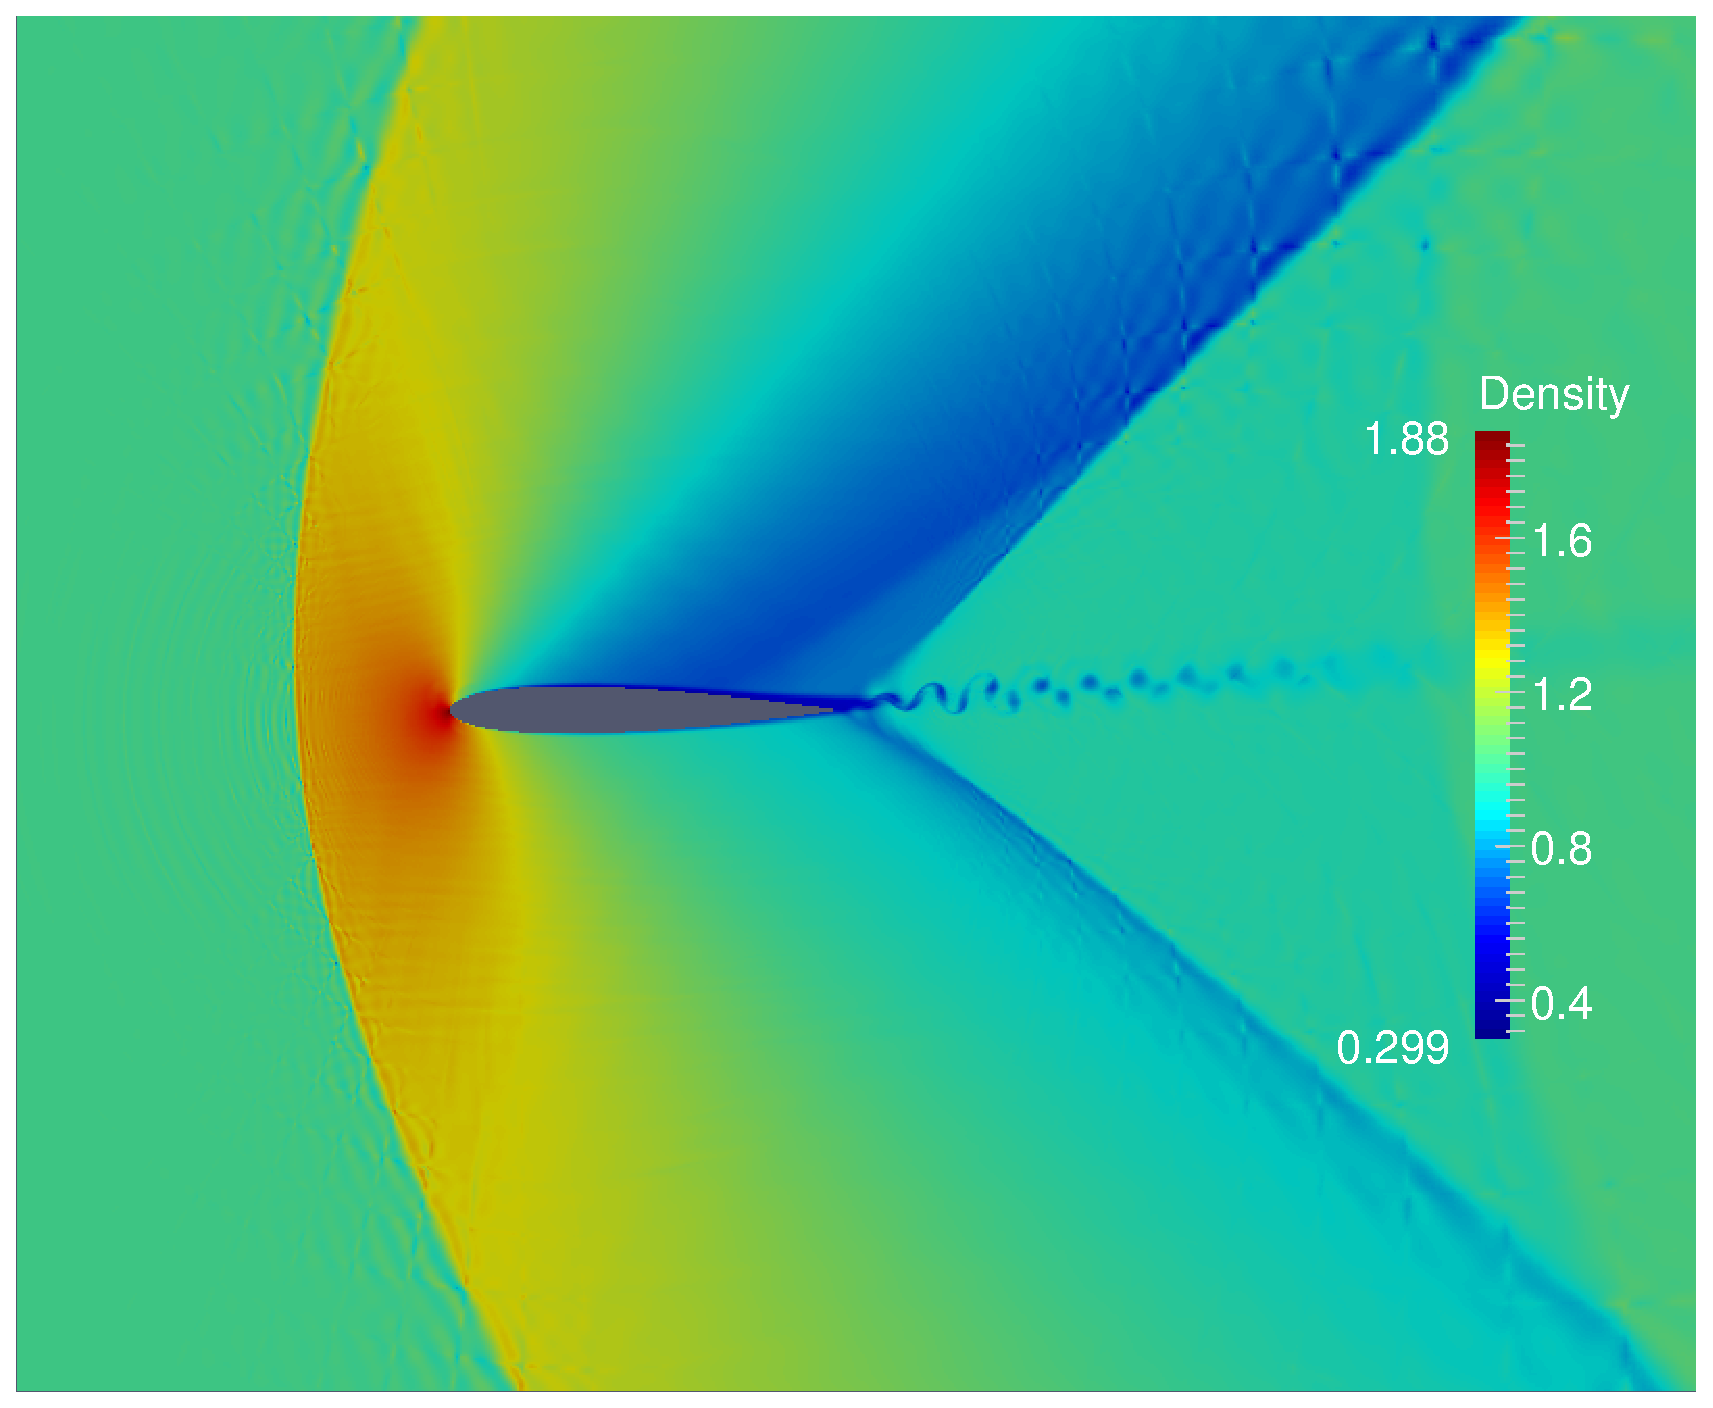
\includegraphics[width=.85\linewidth]{./figures/density-t1050010-jet}
  \captionof{figure}{density contours respectively for viscous flow at M = 1.2 over a NACA 0012 airfoil at 5$^{\circ}$ AoA with polynomial order 6 (49 points in each element)}
  \label{fig:visM1pt2-density}
\end{minipage}%
\begin{minipage}[t]{.5\textwidth}
  \centering
  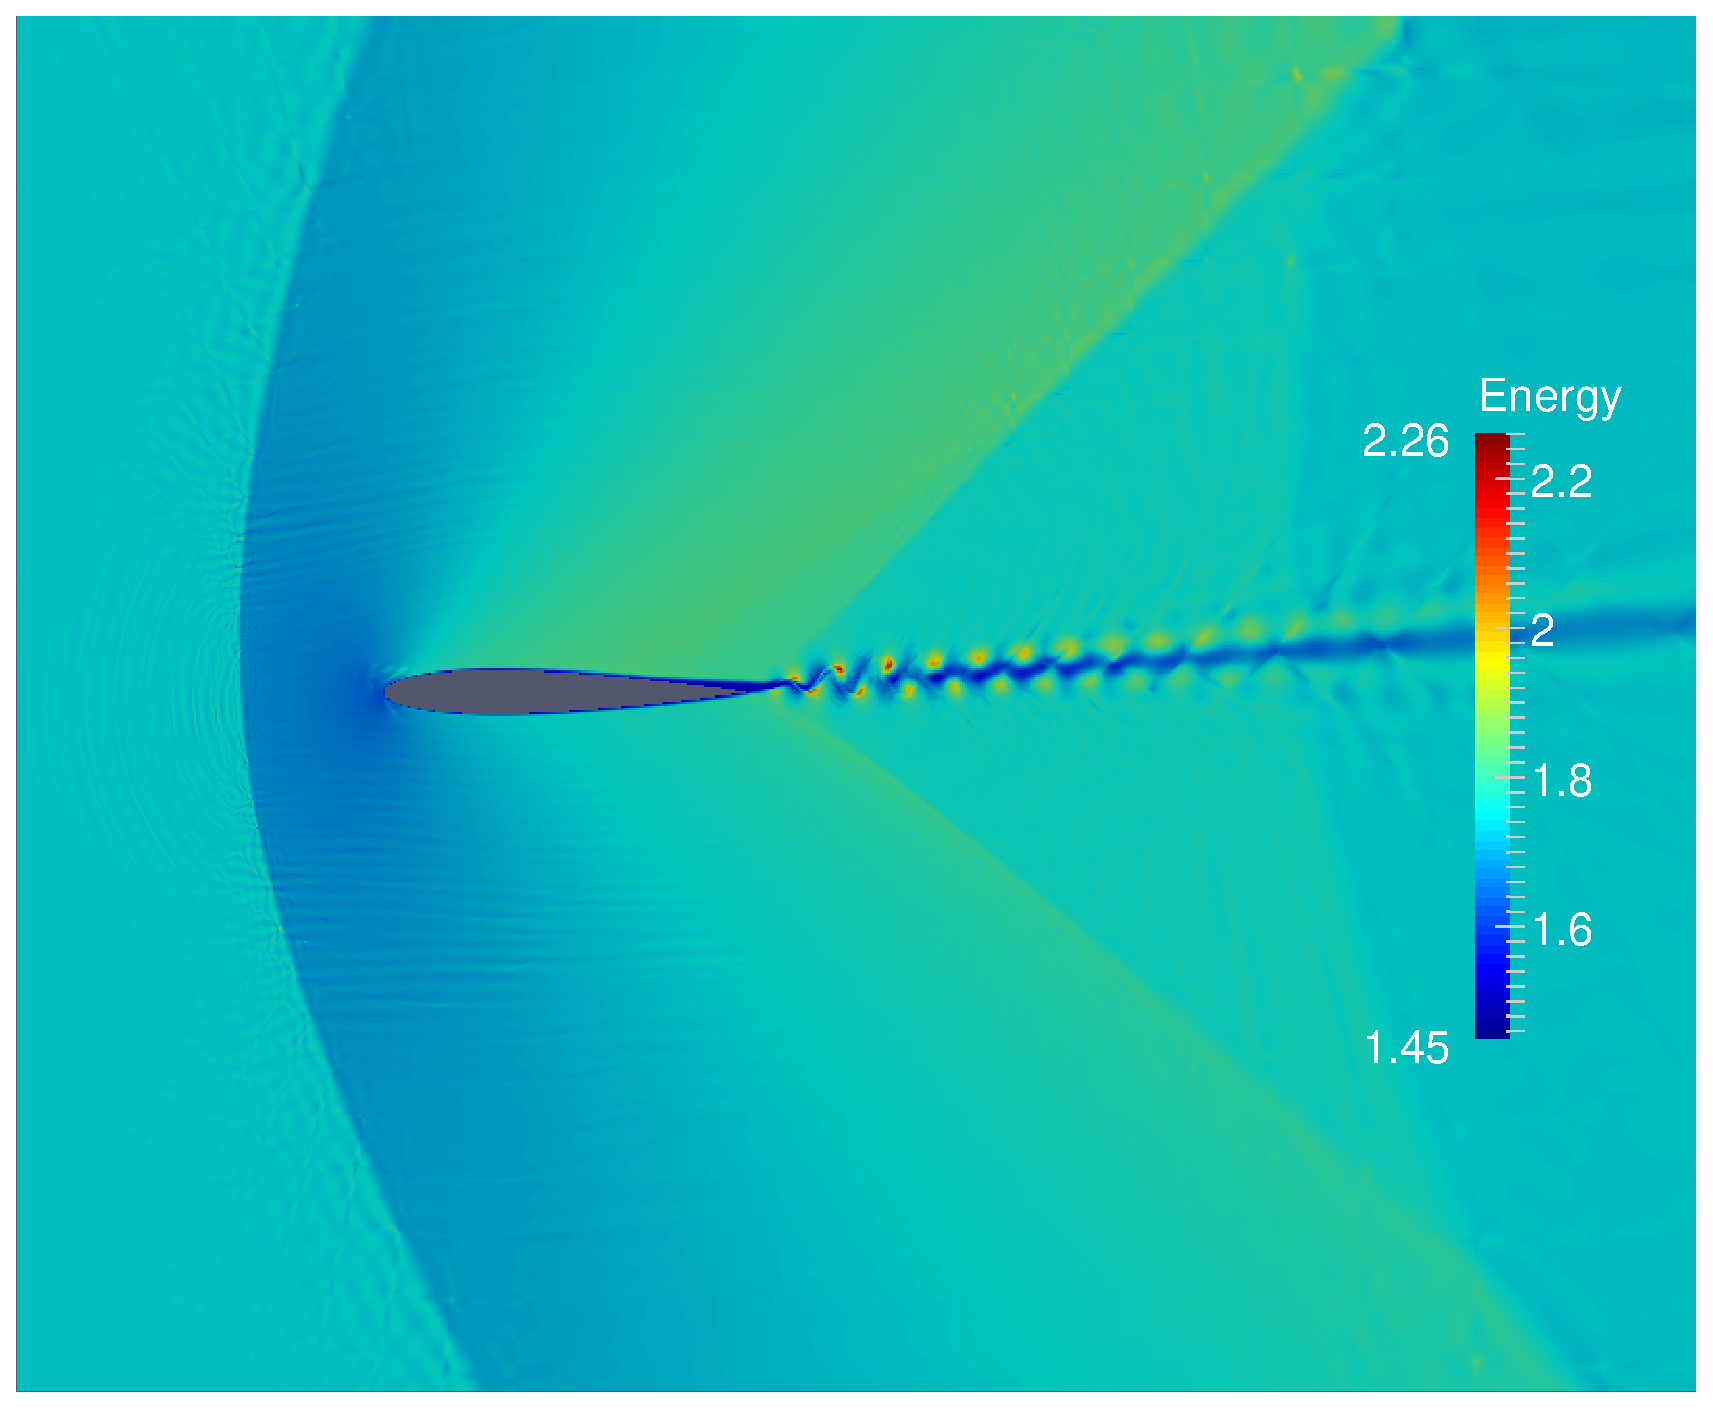
\includegraphics[width=.85\linewidth]{./figures/energy-t1050010-jet}
  \captionof{figure}{Energy contours}
  \label{fig:visM1pt2-energy}
\end{minipage}
\end{figure} 

\begin{figure}[h] \tt
\centering
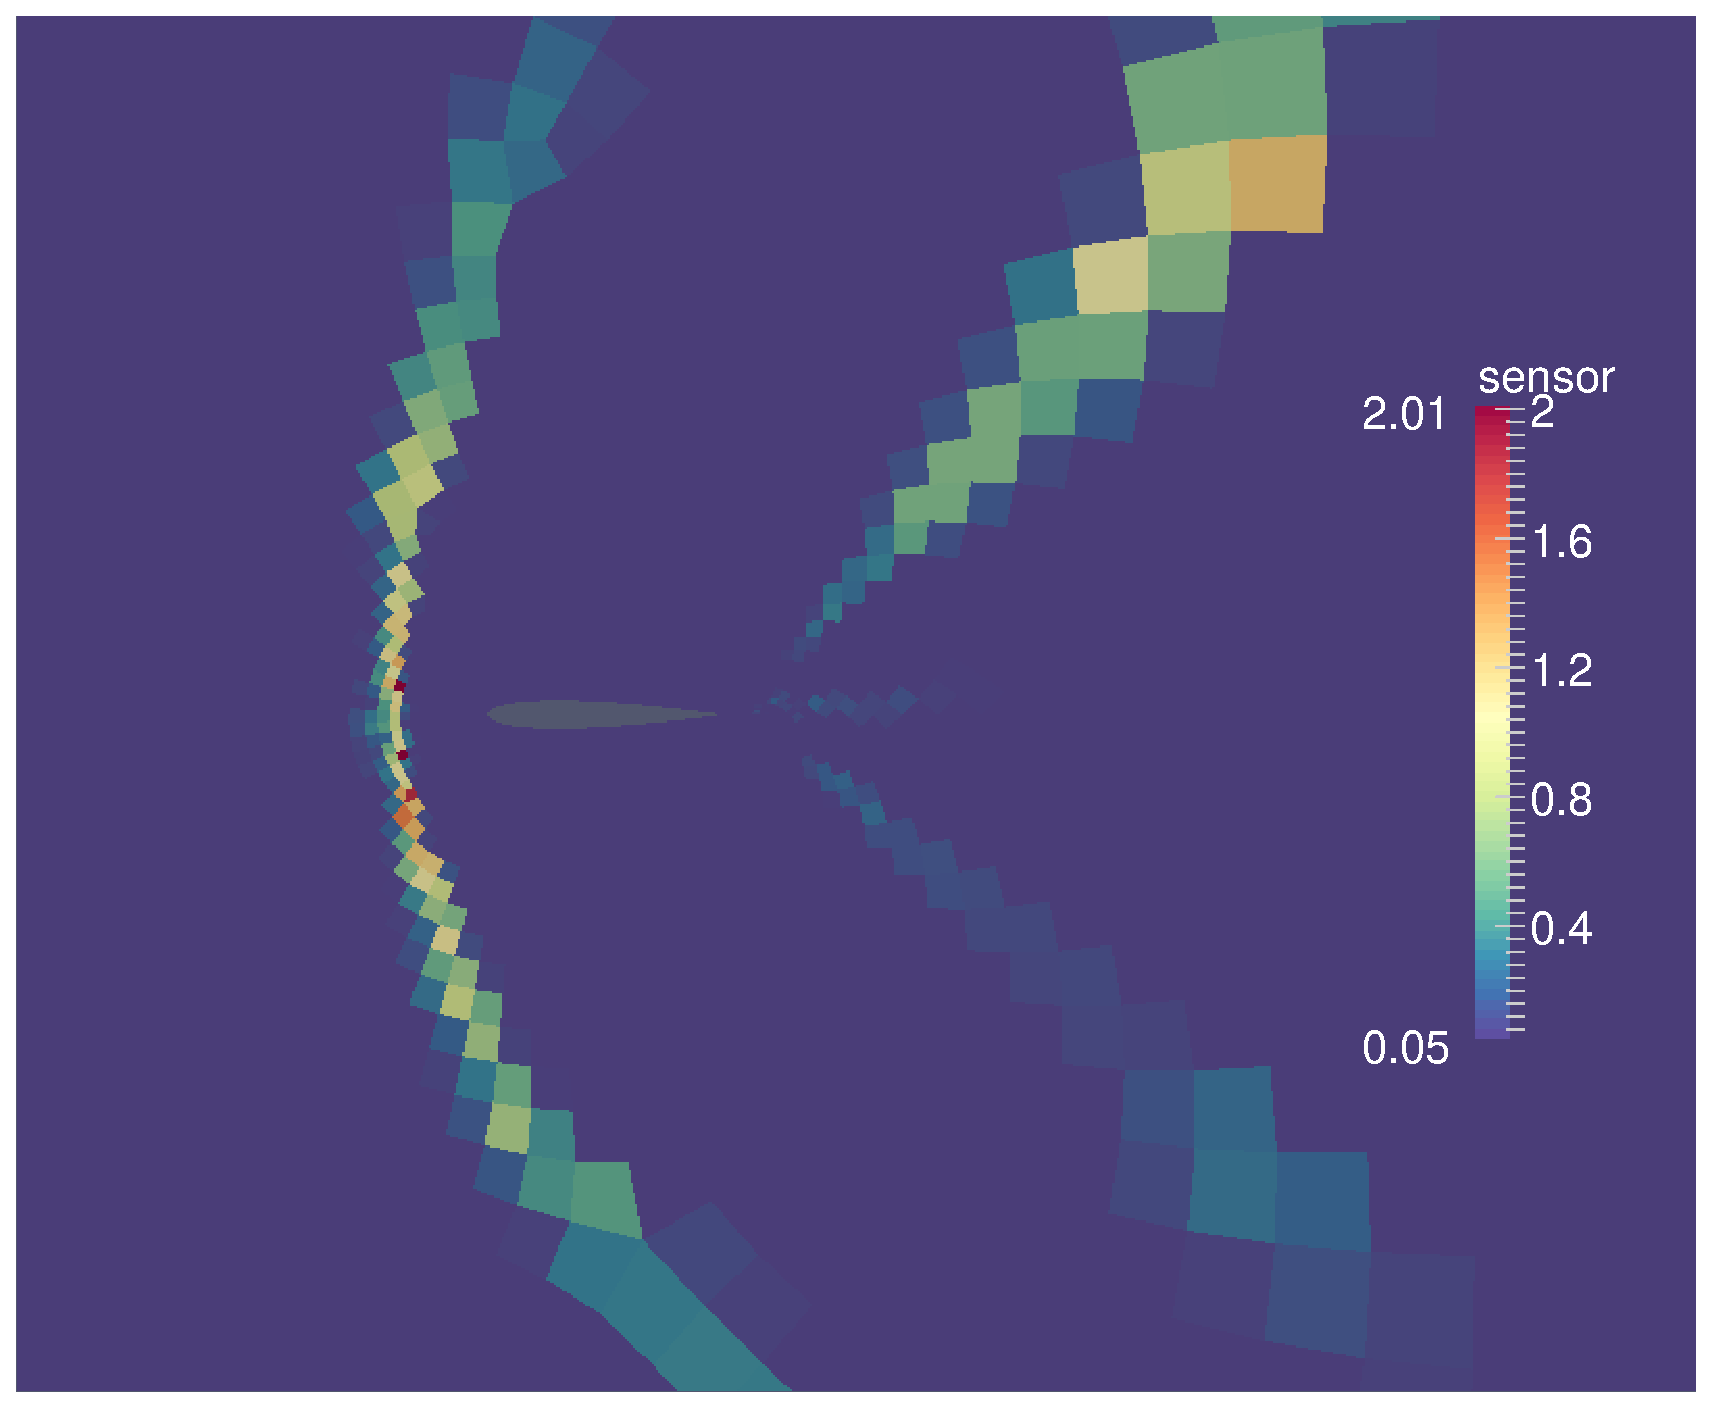
\includegraphics[angle=0, scale = 0.55]{./figures/sensor-t1050010-spectral}
\caption{Figure shows the elemental shock "sensor" for the M = 1.2 viscous case shown in figure ~\ref{fig:visM1pt2-density}. The shock sensor is just the maximum value of the enhanced kernel in each element}
\label{fig:sensor}
\end{figure}

\begin{figure}[h] \tt
\centering
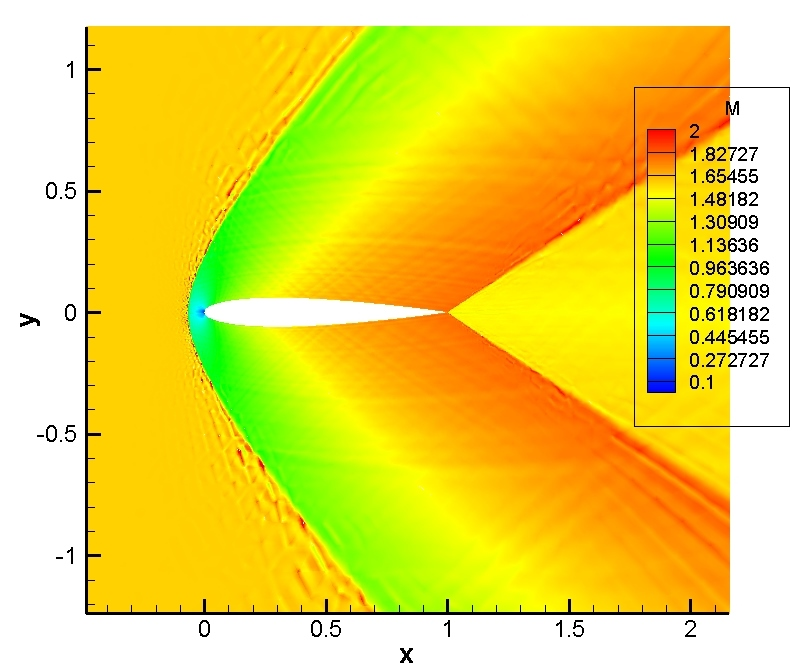
\includegraphics[angle=0, scale = 0.68]{./figures/M1pt6order3-inv-720ktime-mach.jpg} \\
\caption{Mach contours for inviscid flow over Naca0012 at M = 1.6 and AoA = $0^{\circ} $ on a triangle-mesh using Persson and Peraire's method and using artificial viscosity}
\label{fig:inv_mach}
\end{figure}

\begin{figure}
\centering
\begin{minipage}[t]{.55\textwidth}
  \centering
  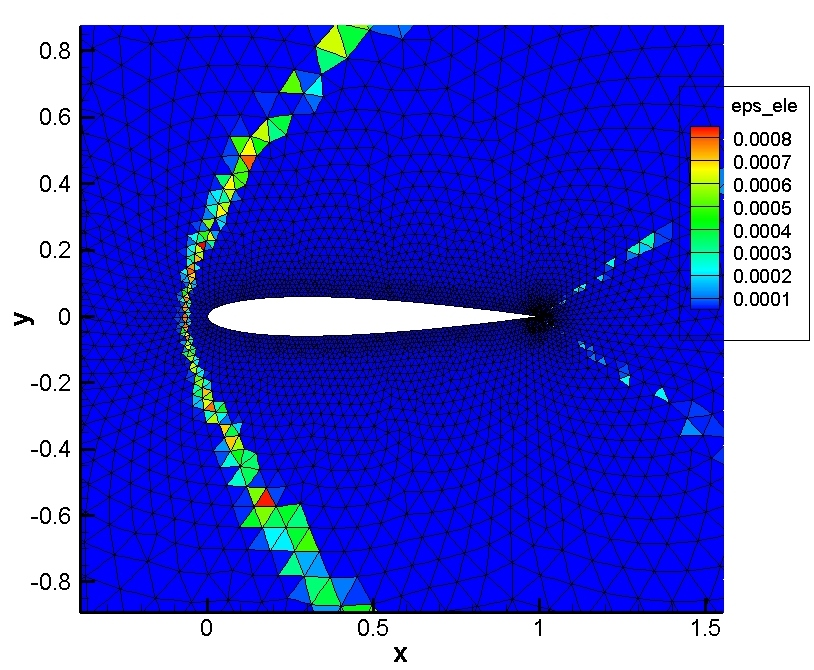
\includegraphics[width=.85\linewidth]{./figures/M1pt6-inv-av-ele-mesh}
  \captionof{figure}{Element-wise AV co-efficients for the inviscid M 1.6 case}
  \label{fig:AV-ele}
\end{minipage}%
\begin{minipage}[t]{.55\textwidth}
  \centering
  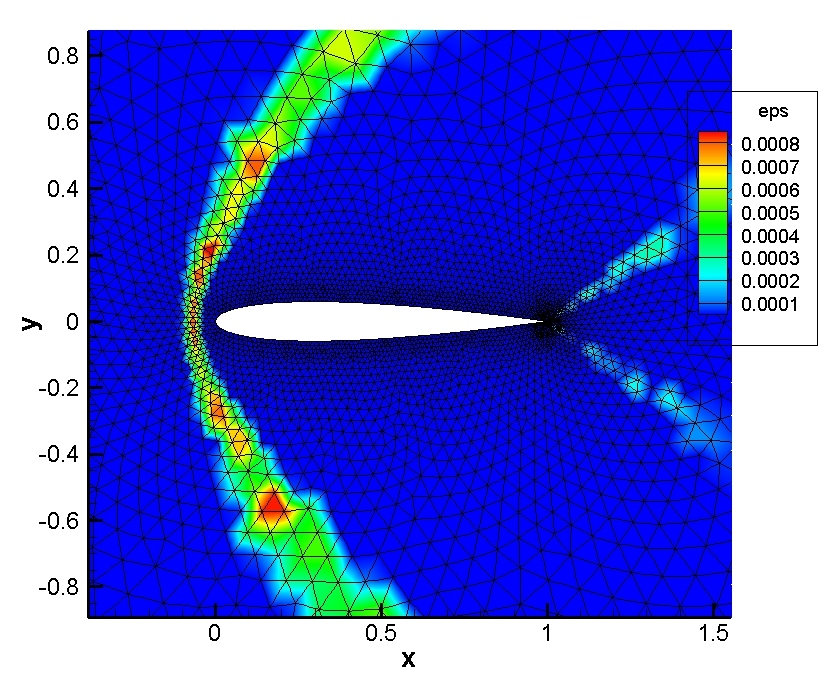
\includegraphics[width=.85\linewidth]{./figures/M1pt6-inv-av-mesh}
  \captionof{figure}{AV co-efficients with continuity enforcement}
  \label{fig:AV-cont}
\end{minipage}
\end{figure} 

\subsection{Spalart-Allmaras (SA) Turbulence Model and Negative $\tilde\nu$ Modification}

The one equation SA turbulence model is one of the more commonly used turbulence models used to solve attached and moderately separated aerodynamic flows \cite{spalart1992one}. The added equation directly solves for turbulent eddy viscosity via advection, diffusion, production and dissipation. A modified form of the equation can be written as \cite{burgess2012robust,oliver2008high,moro2011navier}:
\begin{align}
	\frac{\partial}{\partial t}(\rho\tilde\nu) + \nabla\cdot(\rho\tilde\nu\boldsymbol{u}) = c_{b_1}\tilde S \rho\nu\psi + \frac{1}{\sigma}\left[\nabla\cdot((\mu + \mu\psi)\nabla\tilde\nu) + c_{b_2}\rho\nabla\tilde\nu\cdot\nabla\tilde\nu\right] - c_{w_1}\rho f_w \left(\frac{\nu\psi}{d}\right)^2
\end{align}

where $\tilde\nu$ is a modified version of the kinematic eddy viscosity and $\nu$ is the kinematic viscosity. The other variables are defined as:

\begin{align}
	 \mu_t =
	  \begin{cases}
	   \rho\tilde\nu f_{v_1} & \text{if } \tilde\nu \ge 0 \\
	   0       & \text{if } \tilde\nu < 0
	  \end{cases}
	  \quad \mbox{where} \quad f_{v_1} = \frac{\left(\frac{\rho\tilde\nu}{\mu}\right)^3}{\left(\frac{\rho\tilde\nu}{\mu}\right)^3 + c_{v_1}^3}
\end{align}

\begin{align}
	\tilde S &=
	\begin{cases}
	   S + \bar S & \text{if } \bar S \ge -c_{v_2}S \\
	   S + \frac{S(c_{v_2}^2 S + c_{v_3}\bar S)}{(c_{v_3} - 2c_{v_2})S - \bar S} & \text{if } \bar S \le -c_{v_2}S
	\end{cases}
\end{align}
\begin{align}
	S &= \sqrt{\boldsymbol{\omega}\cdot\boldsymbol{\omega}}
	\qquad \bar S = \frac{(\nu\psi)^2 f_{v_2}}{\kappa^2 d^2} \\
	f_{v_2} &= 1 - \frac{\psi}{1 + \psi f_{v_1}}
\end{align}

\begin{align}
	f_w &= g\left[\frac{1 + c_{w_3}^6}{g^6 + c_{w_3}^6}\right]^{1/6} 
	\qquad g = r + c_{w_2}(r^6 - r) 
	\qquad r = \frac{\nu\psi}{\tilde S \kappa^2 d^2}
\end{align}

where S is the magnitude of vorticity, d is the closest distance to a wall, $c_{b1} = 0.1355$, $\sigma = \frac{2}{3}$, $c_{b2} = 0.622$, $K = 0.41$, $\text{Pr}_t = 0.9$, $c_{v1} = 7.1$, $c_{v2} = 0.7$, $c_{v3} = 0.9$, $c_{w1} = \frac{c_{b1}}{K^2} + \frac{(1+c_{b2})}{\sigma}$, $c_{w2} = 0.3$, $c_{w3} = 2$.\\

The diffusion term, $\nabla\cdot(\rho\tilde\nu\boldsymbol{u})$, may become discontinuous in the first derivative leading to oscillations in high-order polynomials. This can lead to large negative values of the modified eddy viscosity term, $\tilde\nu$, significant enough to cause an unbounded solution. To prevent this, the following modification is introduced \cite{moro2011navier}.
\begin{align}
	\psi &=
	\begin{cases}
	   0.05log(1.0 + e^{(20.0\chi)}) & \text{if } \chi \le 10.0, \\
	   \chi & \text{if } \chi > 10.0,
	\end{cases} \\
	\chi &= \frac{\tilde\nu}{\nu}
\end{align}

\subsection{Large Eddy Simulation}\label{lesmodels}

In order to resolve all the scales of motion in a high Reynolds number turbulent flow, the computational mesh would have to be exceedingly fine.
A practical solution is to employ the Large Eddy Simulation (LES) formulation, which only resolves the larger scales of motion and thus allows for the use of coarser meshes.

The effect of the unresolved or subgrid-scale (SGS) dynamics on the solution is accounted for by an SGS model for the subgrid-scale stress $\tau_{ij}$, which is added to the viscous stress tensor $\sigma_{ij}$ given by (\ref{sigma}):

\begin{eqnarray}\label{tausgs}
\sigma_{ij} &&= 2 \mu S^d_{ij} + \tau_{ij},\\
S^d_{ij} &&= \frac 1 2 \l( \frac{\partial u_i}{\partial x_j} + \frac{\partial u_j}{\partial x_i} - \frac{2}{3} \delta_{ij}\frac{\partial u_k}{\partial x_k} \r).
\end{eqnarray}

The standard Smagorinsky model\cite{smagorinsky1963} is available in HiFiLES:
\begin{eqnarray}\label{smag}
\tau_{ij} &&= 2 \mu_t S^d_{ij}, \\
\mu_t &&= \rho C_S^2 \bigtriangleup^2 | S^d |,\\
| S^d | &&= \sqrt{2 S^d_{ij} S^d_{ij}},
\end{eqnarray}
where $\mu_t$ is the eddy viscosity, $C_S = 0.1$ is the Smagorinsky coefficient and $\bigtriangleup$ is the filter width. In HiFiLES the filter width is given by (in 3D):
\begin{equation}
\bigtriangleup = \alpha (\text{vol})^{1/3},
\end{equation}
where $\alpha \geq 1$ is a user-defined scaling factor and vol is the element volume.

HiFiLES also includes the Wall-Adapting Local Eddy-Viscosity (WALE) model~\cite{nicoud1999} and the Similarity model~\cite{bardina1980}.
The Similarity model incorporates a low-pass filtering operator, for which several choices are available in HiFiLES: a discrete Gaussian filter\cite{lodato2012b}, a high-order commuting Vasilyev-type filter\cite{vasilyev1998,vasilyev2001} and a modal Vandermonde-type filter\cite{blackburn2003}.

The modal filter can be used on unstructured tetrahedral meshes. For details of these operators, see Lodato, Castonguay and Jameson~\cite{lodato2012b} and Bull and Jameson~\cite{bull2013a}. One can combine the similarity model with the Smagorinsky or WALE model to form a mixed SGS model. The WALE-similarity mixed (WSM) model, first proposed by Lodato et al.~\cite{lodato2009}, was used in simulations of the flow over a square cylinder (see Section \ref{sqcyl}).

\subsection{Computing Architecture and Scalability}

The HiFiLES code has been designed to work on multi-CPU as well as multi-CPU-GPU platforms. The Flux Reconstruction method in its current form with explicit time-stepping has a great potential for parallelization. Since the solution points are not explicitly shared between elements, most of the computations are element-local enabling an efficient use of shared memory on GPUs. Also, several computations are independent for each solution point and the highly parallelizable nature of GPUs becomes very useful. A detailed description of the parallelization of the FR method, along with scalability and performance analysis has been performed in \cite{castonguay2011}.
%mention strong/weak scaling results if time


% !TEX root = ./main.tex

\section{Verification and Validation}

\label{sec:verification}

% Manufactured solutions
% !TEX root = ./main.tex
\graphicspath{{figures_manufactured/}}% Set graphics path location


\subsection{Method of Manufactured Solutions}

This section describes the test of HiFiLES's spatial order of accuracy using the Method of Manufactured Solutions (MMS) in 2D and 3D for viscous flows. As shown by Salari et. al\cite{salari2000code}, the MMS test rigorously assesses the correctness of implementation of a solver of Partial Differential Equations. Simplex elements are crucial for simulations in unstructured meshes and have a more complex implementation than squares and hexahedra. As a result, we perform the MMS test in grids using simplex elements.

The MMS test for NS solvers requires checking the solver's solution against an exact solution. Such exact solution can be chosen arbitrarily. The NS equations can be satisfied with this arbitrary solution by including a time-dependent source term in the equations. Then, we solve

\begin{equation}
\frac{\partial U}{\partial t} +  \nabla \cdot {\bf F} = S
\end{equation}

For the following tests, we selected a smooth exact solution, so aliasing does not pollute the results. We picked

\begin{equation}\label{eq:NSwithSource}
U_{2D} = \l(
\begin{tabular}{c}
$\sin{(k(x+y) - \omega t)} + a$\\
$\sin{(k(x+y) - \omega t)} + a$\\
$\sin{(k(x+y) - \omega t)} + a$\\
$(\sin{(k(x+y) - \omega t)} + a)^2$
\end{tabular}
\r) \;\; 
U_{3D} = \l(
\begin{tabular}{c}
$\sin{(k(x+y+z) - \omega t)} + a$\\
$\sin{(k(x+y+z) - \omega t)} + a$\\
$\sin{(k(x+y+z) - \omega t)} + a$\\
$\sin{(k(x+y+z) - \omega t)} + a$\\
$(\sin{(k(x+y+z) - \omega t)} + a)^2$
\end{tabular}
\r)
\end{equation}

To find the value of $S$, we plug the values of our selected $U$ into the left-hand side of Equation~\eqref{eq:NSwithSource} and simplify. The resulting expression is $S$. 
We let Pr$=0.72, \gamma = 1.4, k = \pi, \omega = \pi, a = 3.0$ and $\mu = 0.001$.

The meshes used have dimensions $[-1,1] \times [-1,1]$ in 2D and $[-1,1] \times [-1,1] \times [-1,1]$ in 3D. Periodic boundary conditions were applied on the boundaries of the square and cube domains. Uniform square and cubic meshes were created and then each element was subdivided into triangles or tetrahedra. Two triangles were created from each square, and six tetrahedra were created from each cube. Consequently, in 2D a $N \times N$ mesh contains $2N^2$ triangles, and in 3D a $N \times N \times N$ mesh contains $6N^3$ tetrahedra. 

In 3D, the time step was $1$e$-4$ seconds and 10 seconds of flow were simulated. In 2D, the time step was $1$e$-6$ seconds and 1 second of flow was simulated. The time-stepping scheme used was the low-storage, $4^\text{th}$ order accurate RK45 method.


\begin{table}[h]
\centering
\begin{tabular}{ c c c c c c c} 
  
 Mesh: &   & 2x2x2 & 4x4x4 & 8x8x8 & 16x16x16 & Overall Order \\ 
 \hline 
 \multirow{2}{*}{$p = 1$} & $L_2$ error & 5.76e-01 & 1.35e-01 & 3.22e-02 & 7.90e-03 &   \\ 
  
   & $\mathcal{O}(L_2)$ &   & 2.10 & 2.06 & 2.03 & 2.06 \\ 
 \hline 
 \multirow{2}{*}{$p = 2$} & $L_2$ error & 4.09e-01 & 5.52e-02 & 6.87e-03 & 8.53e-04 &   \\ 
  
   & $\mathcal{O}(L_2)$ &   & 2.89 & 3.01 & 3.01 & 2.97 \\ 
 \hline 
 \multirow{2}{*}{$p = 3$} & $L_2$ error & 9.77e-02 & 5.97e-03 & 3.78e-04 &   &   \\ 
  
   & $\mathcal{O}(L_2)$ &   & 4.03 & 3.98 &   & 4.01 \\ 
 \hline 
 \multirow{2}{*}{$p = 4$} & $L_2$ error & 1.12e-02 & 6.39e-04 & 2.07e-05 &   &   \\ 
  
   & $\mathcal{O}(L_2)$ &   & 4.13 & 4.95 &   & 4.54 \\ 
 \hline 
 \multirow{2}{*}{$p = 5$} & $L_2$ error & 1.53e-01 & 5.08e-03 & 6.92e-05 &   &   \\ 
  
   & $\mathcal{O}(L_2)$ &   & 4.91 & 6.20 &   & 5.55 \\ 
 \hline 
 \end{tabular}
\caption{Tets error1} 
 \end{table}

\begin{table}[H]
\centering
\begin{tabular}{ c c c c c c c} 
  
 Polynomial Order & Mesh: & 2x2x2 & 4x4x4 & 8x8x8 & 16x16x16 & Overall Order of Accuracy \\ 
 \hline 
 \multirow{2}{*}{$p = 1$} & $L_2$ error & 1.98e+01 & 9.57e+00 & 4.55e+00 & 2.19e+00 &   \\ 
  
   & $\mathcal{O}(L_2)$ &   & 1.05 & 1.07 & 1.06 & 1.06 \\ 
 \hline 
 \multirow{2}{*}{$p = 2$} & $L_2$ error & 1.17e+01 & 2.98e+00 & 7.10e-01 & 1.71e-01 &   \\ 
  
   & $\mathcal{O}(L_2)$ &   & 1.97 & 2.07 & 2.06 & 2.03 \\ 
 \hline 
 \multirow{2}{*}{$p = 3$} & $L_2$ error & 3.17e+00 & 3.81e-01 & 4.73e-02 &   &   \\ 
  
   & $\mathcal{O}(L_2)$ &   & 3.06 & 3.01 &   & 3.03 \\ 
 \hline 
 \multirow{2}{*}{$p = 4$} & $L_2$ error & 5.21e-01 & 4.27e-02 & 2.69e-03 &   &   \\ 
  
   & $\mathcal{O}(L_2)$ &   & 3.61 & 3.99 &   & 3.80 \\ 
 \hline 
 \multirow{2}{*}{$p = 5$} & $L_2$ error & 3.20e+00 & 1.88e-01 & 4.79e-03 &   &   \\ 
  
   & $\mathcal{O}(L_2)$ &   & 4.09 & 5.29 &   & 4.69 \\ 
 \hline 
 \end{tabular}
\caption{Accuracy of HiFiLES for NS equations with source term in tetrahedral meshes at $t = 10$. $L_2$ error is the $L_2$-norm of the error in the gradient of the energy field:$\frac{\partial}{\partial x_i} (\rho e)$}
\label{table:tetsError2} 
 \end{table}

\begin{table}[h]
\centering
\begin{tabular}{ c c c c c c c c} 
  
 Mesh: &   & 4x4 & 8x8 & 16x16 & 32x32 & 64x64 & Overall Order \\ 
 \hline 
 \multirow{2}{*}{$p = 1$} & $L_2$ error & 7.92e-01 & 1.84e-01 & 4.36e-02 & 1.07e-02 & 2.68e-03 &   \\ 
  
   & $\mathcal{O}(L_2)$ &   & 2.10 & 2.08 & 2.03 & 2.00 & 2.05 \\ 
 \hline 
 \multirow{2}{*}{$p = 2$} & $L_2$ error & 1.29e-01 & 1.61e-02 & 1.95e-03 & 2.33e-04 & 2.86e-05 &   \\ 
  
   & $\mathcal{O}(L_2)$ &   & 3.00 & 3.05 & 3.06 & 3.03 & 3.04 \\ 
 \hline 
 \multirow{2}{*}{$p = 3$} & $L_2$ error & 1.01e-02 & 9.25e-04 & 5.71e-05 & 3.65e-06 & 2.35e-07 &   \\ 
  
   & $\mathcal{O}(L_2)$ &   & 3.45 & 4.02 & 3.97 & 3.96 & 3.88 \\ 
 \hline 
 \multirow{2}{*}{$p = 4$} & $L_2$ error & 2.60e-03 & 6.33e-05 & 2.00e-06 & 6.49e-08 & 3.62e-09 &   \\ 
  
   & $\mathcal{O}(L_2)$ &   & 5.36 & 4.98 & 4.95 & 4.16 & 4.88 \\ 
 \hline 
 \multirow{2}{*}{$p = 5$} & $L_2$ error & 7.15e-05 & 3.87e-06 & 6.31e-08 &   &   &   \\ 
  
   & $\mathcal{O}(L_2)$ &   & 4.21 & 5.94 &   &   & 5.07 \\ 
 \hline 
 \end{tabular}
\caption{Tris error1} 
 \end{table}

\begin{table}[H]
\centering
\begin{tabular}{ c c c c c c c c} 
  
 Mesh: &   & 4x4 & 8x8 & 16x16 & 32x32 & 64x64 & Overall Order \\ 
 \hline 
 \multirow{2}{*}{$p = 1$} & $L_2$ error & 1.61e+01 & 8.31e+00 & 3.81e+00 & 1.71e+00 & 7.84e-01 &   \\ 
  
   & $\mathcal{O}(L_2)$ &   & 0.96 & 1.12 & 1.15 & 1.13 & 1.10 \\ 
 \hline 
 \multirow{2}{*}{$p = 2$} & $L_2$ error & 4.05e+00 & 8.16e-01 & 1.90e-01 & 4.54e-02 & 1.11e-02 &   \\ 
  
   & $\mathcal{O}(L_2)$ &   & 2.31 & 2.11 & 2.06 & 2.04 & 2.12 \\ 
 \hline 
 \multirow{2}{*}{$p = 3$} & $L_2$ error & 4.71e-01 & 6.39e-02 & 7.03e-03 & 7.75e-04 & 8.84e-05 &   \\ 
  
   & $\mathcal{O}(L_2)$ &   & 2.88 & 3.18 & 3.18 & 3.13 & 3.11 \\ 
 \hline 
 \multirow{2}{*}{$p = 4$} & $L_2$ error & 1.01e-01 & 4.30e-03 & 2.31e-04 & 1.41e-05 & 5.27e-06 &   \\ 
  
   & $\mathcal{O}(L_2)$ &   & 4.56 & 4.22 & 4.04 & 1.42 & 3.67 \\ 
 \hline 
 \multirow{2}{*}{$p = 5$} & $L_2$ error & 5.04e-03 & 2.50e-04 & 7.80e-06 &   &   &   \\ 
  
   & $\mathcal{O}(L_2)$ &   & 4.33 & 5.00 &   &   & 4.67 \\ 
 \hline 
 \end{tabular}
\caption{Tris error2} 
 \end{table}


Tables \eqref{table:tetsError1} and \eqref{table:tetsError1} show the order of accuracy achieved when calculating\eqref{table:tetsError1}

%\begin{figure}
%\centering
%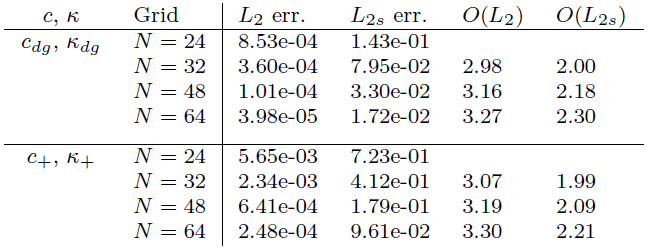
\includegraphics[height=35mm]{table_917} \\
%\caption{Accuracy of ESFR schemes for flow generated by a time-dependent source term on triangular grids, for the case of $p = 2$. The inviscid and viscous numerical fluxes were computed using a Rusanov flux with $\lambda = 1$ and a LDG flux with $\tau = 0.1$ and $\beta = \pm 0.5n$.}
%\label{fig:table_917}
%\end{figure}
%
%\begin{figure}
%\centering
%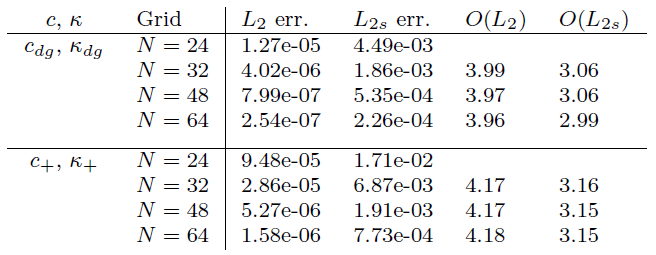
\includegraphics[height=35mm]{table_918} \\
%\caption{Accuracy of ESFR schemes for flow generated by a time-dependent source term on triangular grids, for the case of $p = 3$. The inviscid and viscous numerical fluxes were computed using a Rusanov flux with $\lambda = 1$ and a LDG flux with $\tau = 0.1$ and $\beta = \pm 0.5n$.}
%\label{fig:table_918}
%\end{figure}
%
%\begin{figure}
%\centering
%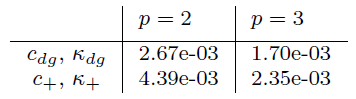
\includegraphics[height=20mm]{table_919} \\
%\caption{Explicit time-step limits ($\Delta t_{max}$) of ESFR schemes for flow generated by a time-dependent source term on the triangular grid with $\tilde{N} = 48$, for the cases of $p = 2$ and $3$. The inviscid and viscous numerical fluxes were computed using a Rusanov flux with $\lambda = 1$ and a LDG flux with $\tau = 0.1$ and $\beta = \pm 0.5n$.}
%\label{fig:table_919}
%\end{figure}
%
%\begin{figure}
%\centering
%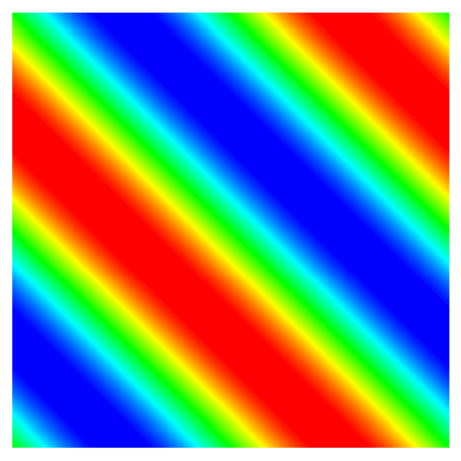
\includegraphics[height=60mm]{figure_912} \\
%\caption{Contours of energy obtained using the ESFR scheme with $c = c_+$ and $\kappa = \kappa_+$ on the triangular grid with $\tilde{N} = 32$ for the case of $p = 3$. The inviscid and viscous numerical fluxes were computed using a Rusanov flux with $\lambda = 1$ and a LDG flux with $\tau = 0.1$ and $\beta = \pm 0.5n$.}
%\label{fig:figure_912}
%\end{figure}
%
%\begin{figure}
%\centering
%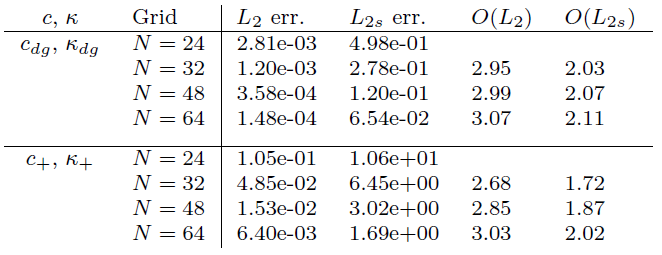
\includegraphics[height=35mm]{table_920} \\
%\caption{Accuracy of ESFR schemes for flow generated by a time-dependent source term on tetrahedral grids, for the case of $p = 2$. The inviscid and viscous numerical fluxes were computed using a Rusanov flux with $\lambda = 1$ and a LDG flux with $\tau = 0.1$ and $\beta = \pm 0.5n$.}
%\label{fig:table_920}
%\end{figure}
%
%\begin{figure}
%\centering
%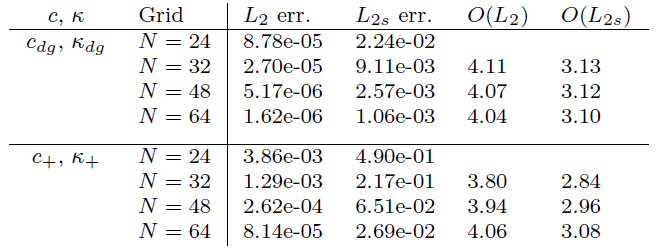
\includegraphics[height=30mm]{table_921} \\
%\caption{Accuracy of ESFR schemes for flow generated by a time-dependent source term on tetrahedral grids, for the case of $p = 3$. The inviscid and viscous numerical fluxes were computed using a Rusanov flux with $\lambda = 1$ and a LDG flux with $\tau = 0.1$ and $\beta = \pm 0.5n$.}
%\label{fig:table_921}
%\end{figure}
%
%\begin{figure}
%\centering
%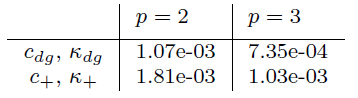
\includegraphics[height=15mm]{table_922} \\
%\caption{Explicit time-step limits ($\Delta t_{max}$) of ESFR schemes for flow generated by a time-dependent source term on the triangular grid with $\tilde{N} = 48$, for the cases of $p = 2 and 3$. The inviscid and viscous numerical fluxes were computed using a Rusanov flux with $\lambda = 1$ and a LDG flux with $\tau = 0.1$ and $\beta = \pm 0.5n$.}
%\label{fig:table_922}
%\end{figure}
%
%\newpage
%\begin{figure}
%\centering
%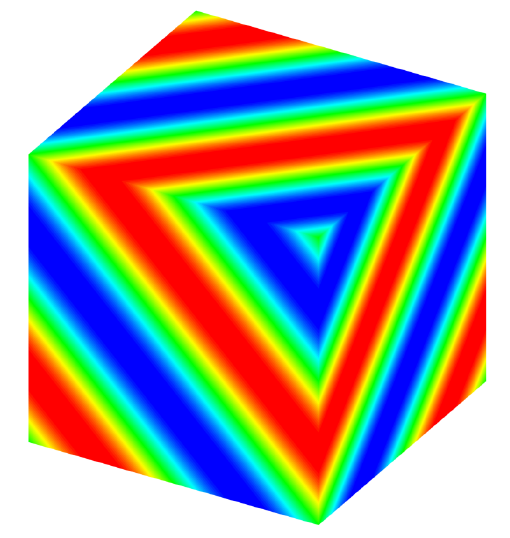
\includegraphics[height=60mm]{figure_913} \\
%\caption{Contours of energy obtained using the ESFR scheme with $c = c_+$ and $\kappa = \kappa_+$ on the tetrahedral grid with $\tilde{N} = 32$ for the case of $p = 3$. The inviscid and viscous numerical fluxes were computed using a Rusanov flux with $\lambda = 1$ and a LDG flux with $\tau = 0.1$ and $\beta = \pm 0.5n$.}
%\label{fig:figure_913}
%\end{figure}


% Flat plate
% !TEX root = ./main.tex
\graphicspath{{figures_flatplate/}}% Set graphics path location

\subsection{Subsonic laminar flat-plate}

Computations of the flow over a subsonic flat-plate have been performed and validated against the Blasius' solution for laminar boundary layer. The flow conditions are Mach number $0.5$, angle of attack $0.0\deg$ and Reynolds number based on the plate length of $1\cdot10^6$. The governing equations are the 2D Navier-Stokes equations with constant ratio of specific heats of $1.4$, Prandtl number of $0.72$ and constant dynamic viscosity of $1.827\cdot 10^{-5} Pa \cdot s$.

\begin{center} 
    \begin{tabular}{l*{5}{c}r}
    Height first cell \& \# of cells inside the boundary layer & Poly order 3 & Poly order 4 & Poly order 5 & Poly order 6 \\ \hline
    Mesh a0 (140 = 14x10). 0.00075 / 2 cells & $\times$ & $\times$ & $\times$ & \Checkmark \\ \hline
    Mesh a1 (560 = 28x20). 0.000375 / 4 cells &  $\times$ & $\times$ & \Checkmark & \Checkmark \\ \hline
    Mesh a2 (2240 = 56x40). 0.0001875  / 8 cells & $\times$ & \Checkmark & \Checkmark & \Checkmark \\ \hline
    Mesh a3 (8960 = 112x80). 0.0000935  / 16 cells & \Checkmark & \Checkmark & \Checkmark & \Checkmark \\
    \hline
    \end{tabular} 
      \captionof{table}{HiFiLES convergence using different grids and polynomial order} \label{table:convergence} 
\end{center}

The objective of this study is to determine the minimum number of elements and the order of polynomial required to converge the flat-plate simulation using HiFILES. In particular, 4 different numerical grids have been used in this study (2, 4, 8, 16 elements inside the boundary layer). The results are summarized in Table \ref{table:convergence}, the simulations require a minimum number of elements in the boundary layer to obtain a satisfactory converge, otherwise, there will be noticeable jumps across the elements.

\begin{figure}
\begin{center}
\begin{minipage}[t]{0.48\columnwidth}
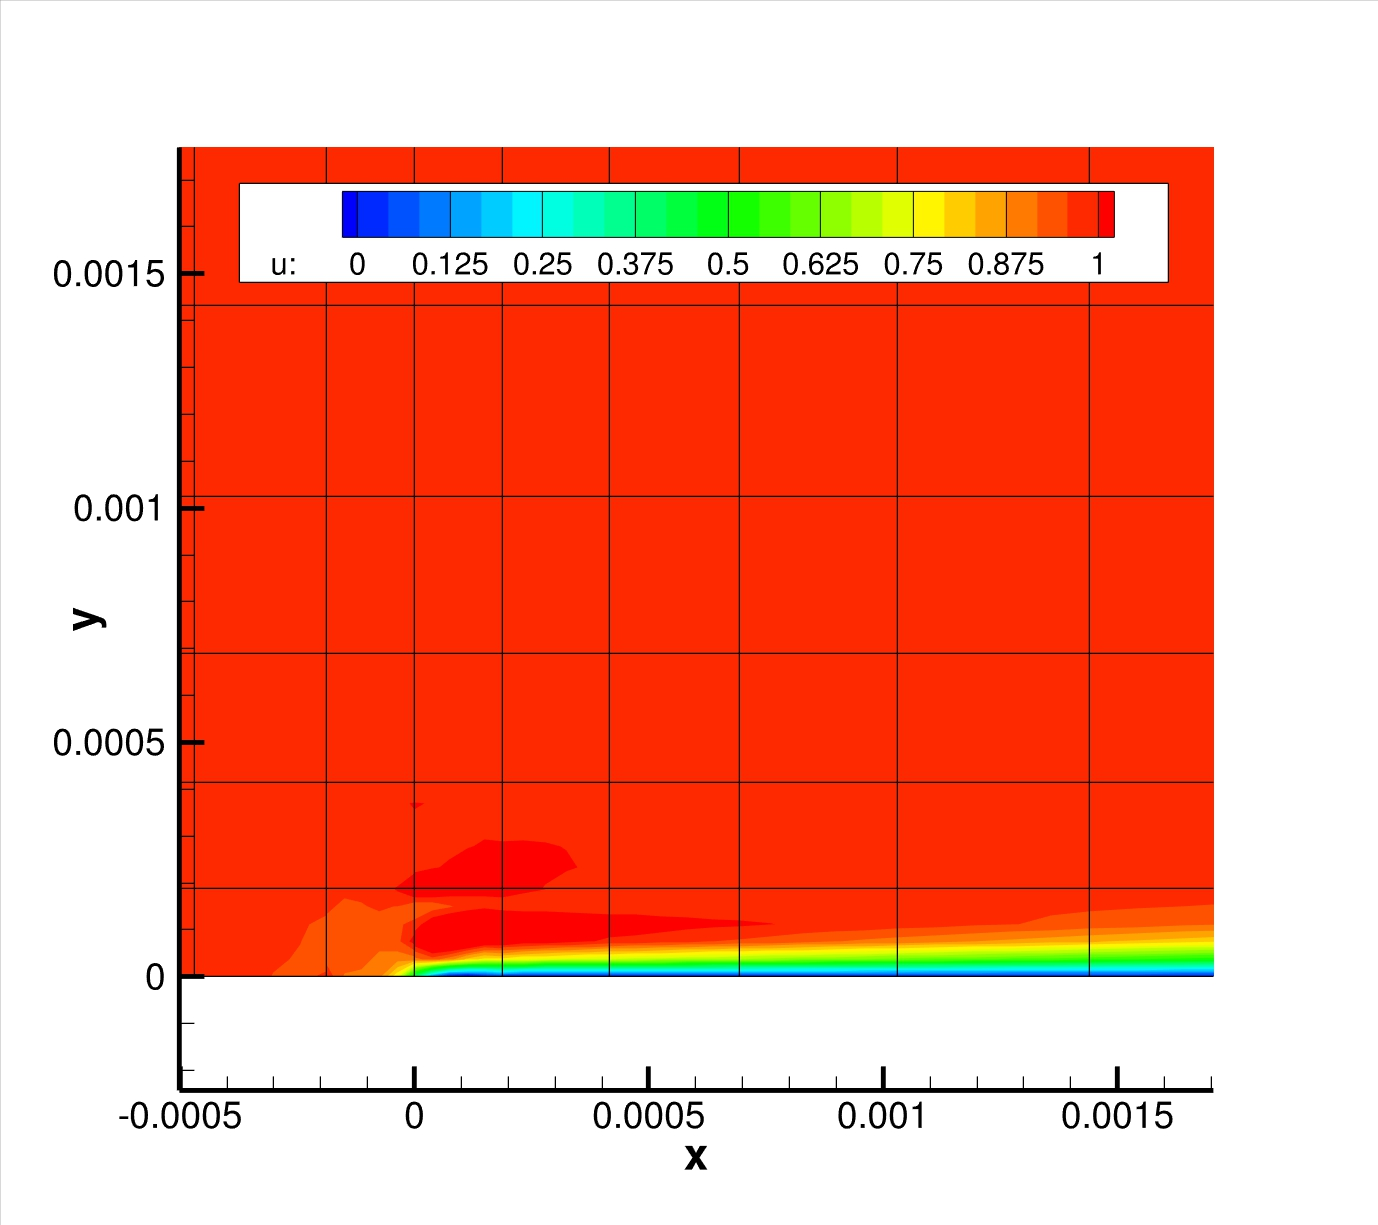
\includegraphics[width = \textwidth,clip=]{LeadingEdge.jpg}
\caption{Detail of the flat-plate leading edge (x=0.0, mesh a2).}
\label{fig:LeagingEdge}
\end{minipage}
\hfill
\begin{minipage}[t]{0.48\columnwidth}
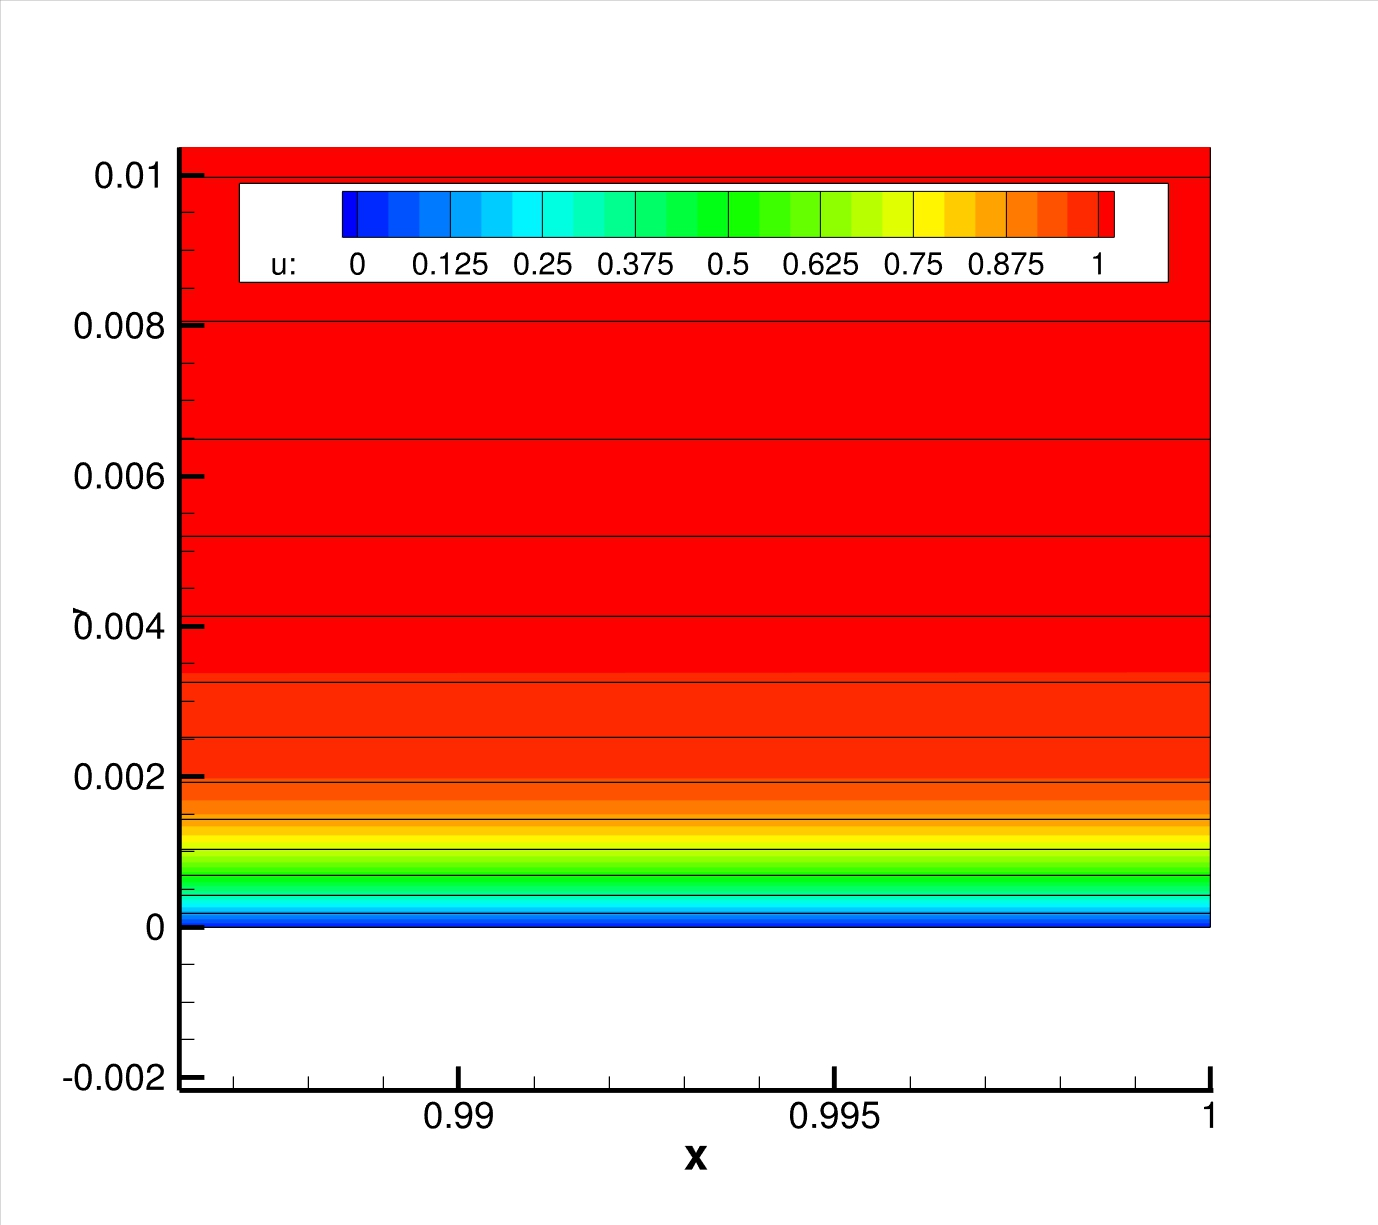
\includegraphics[width = \textwidth,clip=] {EndPlate.jpg}
\caption{Flow solution at the end of the flat-plate (x=1.0, mesh a2).}
\label{fig:TrailingEdge}
\end{minipage}
\end{center}
\end{figure}

The results has been compared with the Blasius' solution for laminar boundary layer with satisfactory results, and some details of the solutions are presented in Fig. \ref{fig:LeagingEdge} (leading edge), and Fig. \ref{fig:TrailingEdge} (end of the flat-plate). It is important to note that in this particular case (mesh a2) the flap-plate is captured using 8 elements, while in a second order solver it would be necessary of the order of ~30 elements inside the boundary layer.

\begin{figure}
\begin{center}
\begin{minipage}[t]{0.48\columnwidth}
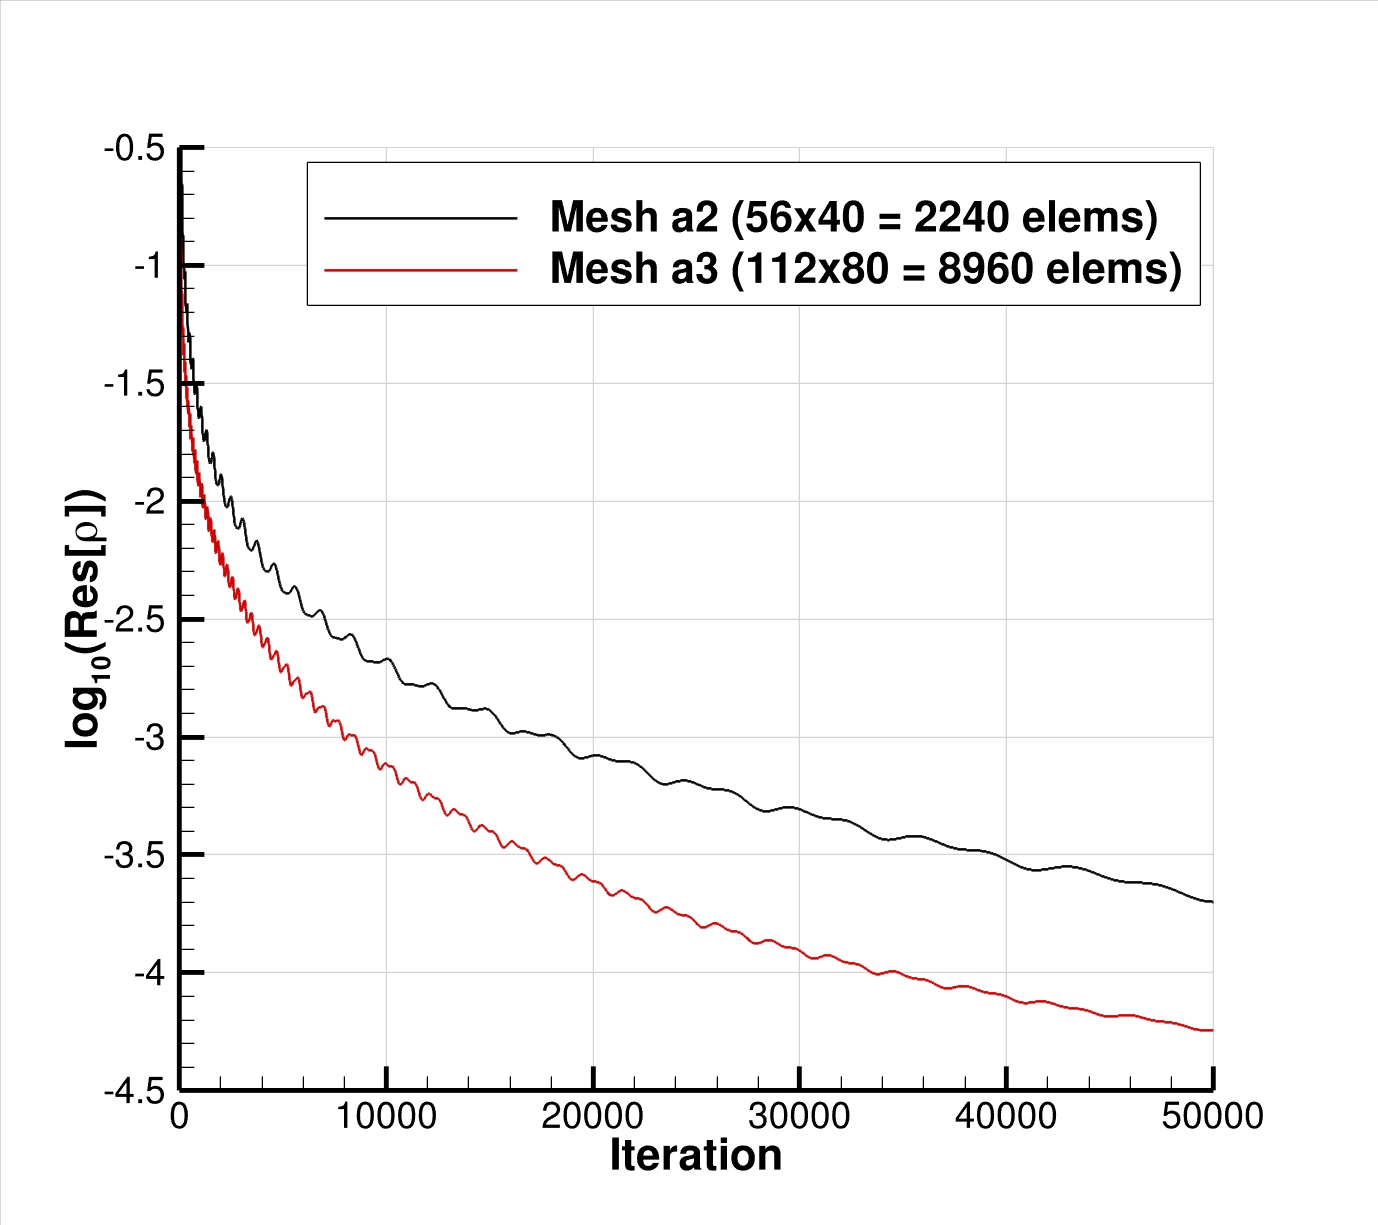
\includegraphics[width = \textwidth,clip=]{CompMesh.jpg}
\caption{Convergence comparison (3$^rd$ order, finest grids).}
\label{fig:ComparisonOrder}
\end{minipage}
\hfill
\begin{minipage}[t]{0.48\columnwidth}
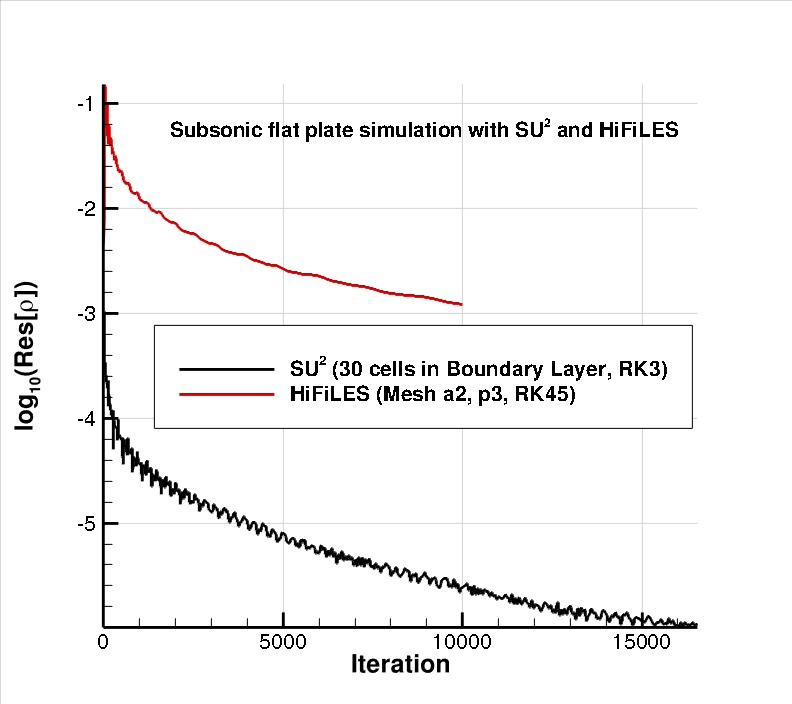
\includegraphics[width = \textwidth,clip=] {CompSu2.jpg}
\caption{Comparison of HiFiLES with SU$^2$ using a similar time integration scheme.}
\label{fig:Comparison_SecondOrder}
\end{minipage}
\end{center}
\end{figure}

To finalize, it is critical to note that the absence of a local time stepping technique in HiFiLES increases the required number of iterations to obtain a converged solution. However, we have noticed an improvement of the rate of converge as we refine the grid (see Fig. \ref{fig:ComparisonOrder}). Finally, the obtained convergence rate is comparable to a second order numerical code (e.g. SU$^2$\cite{palacios13,palacios14}) running using a similar numerical time integration (see Fig.\ref{fig:Comparison_SecondOrder}).


% Circular cylinder
% !TEX root = ./main.tex
\graphicspath{{figures_cylinder/}}% Set graphics path location

\subsection{Circular Cylinder}

The classic test case of laminar flow past a circular cylinder at low Reynolds number has also been chosen as a verification and validation case for the 2D Navier-Stokes equations in HiFiLES, and the results are compared to existing experimental data and simulation results~\cite{park1998}. Two separate cases are computed: first, the steady flow past the cylinder at $Re = 20$, and second, the unsteady flow past the cylinder at $Re = 100$, where the Reynolds number is based upon the diameter of the cylinder. For both cases, the Mach number is set to 0.1 in order to recover nearly incompressible flow for comparisons with the existing incompressible results. The remaining flow conditions are 0$\degr$ angle of attack, a constant ratio of specific heats of $1.4$, a Prandtl number of $0.72$, a free-stream temperature of 300 $K$, and a free-stream dynamic viscosity of $1.853\cdot 10^{-5} Pa \cdot s$ (laminar viscosity varies according to Sutherland's law during the simulation).

The two simulations are performed with third order polynomials on a mesh with 4988 total elements that contains quadrilateral elements near the body of the cylinder and triangular elements out to the far-field. There is a small refinement box immediately downstream of the cylinder to help resolve features in the wake. The rectangular far-field boundaries are located approximately 30 diameters away from the cylinder in the upstream, upward, and downward directions and 50 diameters away in the downstream direction. A view of the mesh near the cylinder surface is show in Fig.~\ref{cylinder_1}.

\begin{figure}
  \begin{subfigmatrix}{2}
    \subfigure[Zoom view of the mesh near the cylinder.]{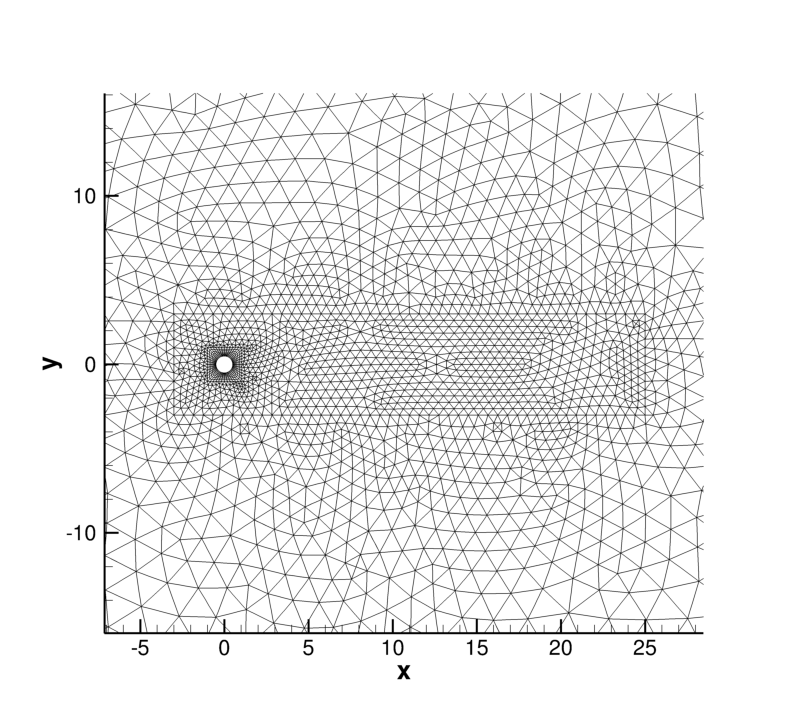
\includegraphics{cylinder_mesh.png}}
    \subfigure[X-velocity contours and streamlines around the circular cylinder for $Re = 20$.]{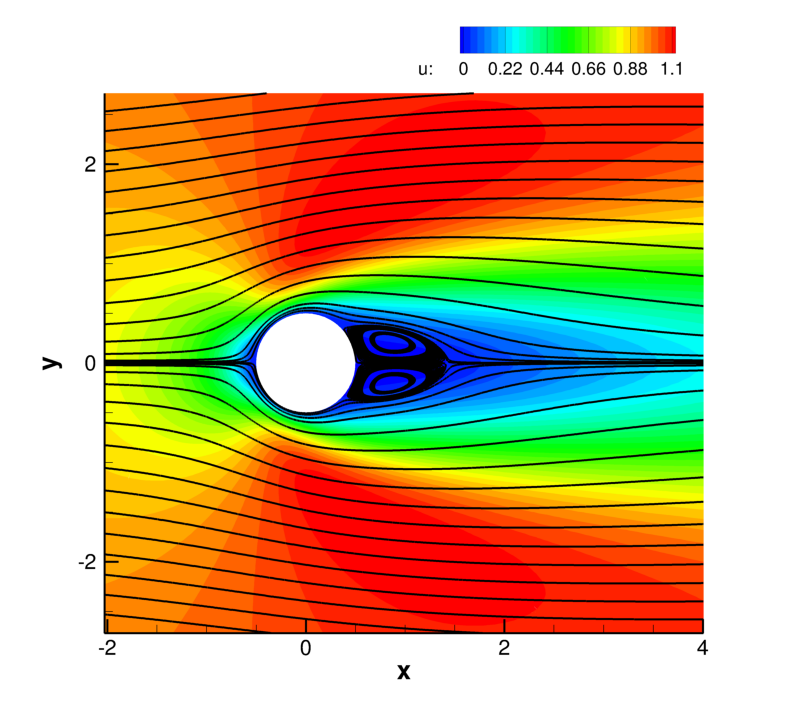
\includegraphics{cylinder_streamlines.png}}
  \end{subfigmatrix}
  \caption{The mesh for the circular cylinder simulations along with x-velocity contours for the $Re = 20$ case.}
  \label{cylinder_1}
\end{figure}

The flow around the cylinder for $Re = 20$ is steady, and it features a large recirculation region behind the cylinder. Fig.~\ref{cylinder_1} presents x-velocity contours around the cylinder along with streamlines. The length of the recirculation region can be determined from the streamlines, and a length of approximately one cylinder diameter agrees well with reported results for $Re = 20$. The coefficient of drag computed by HiFiLES is 2.043, which is close to the value of 2.01 reported by Park et al. Pressure contours around the cylinder are shown in Fig.~\ref{cylinder_2}.

\begin{figure}
  \begin{subfigmatrix}{2}
    \subfigure[Pressure contours for the $Re = 20$ case.]{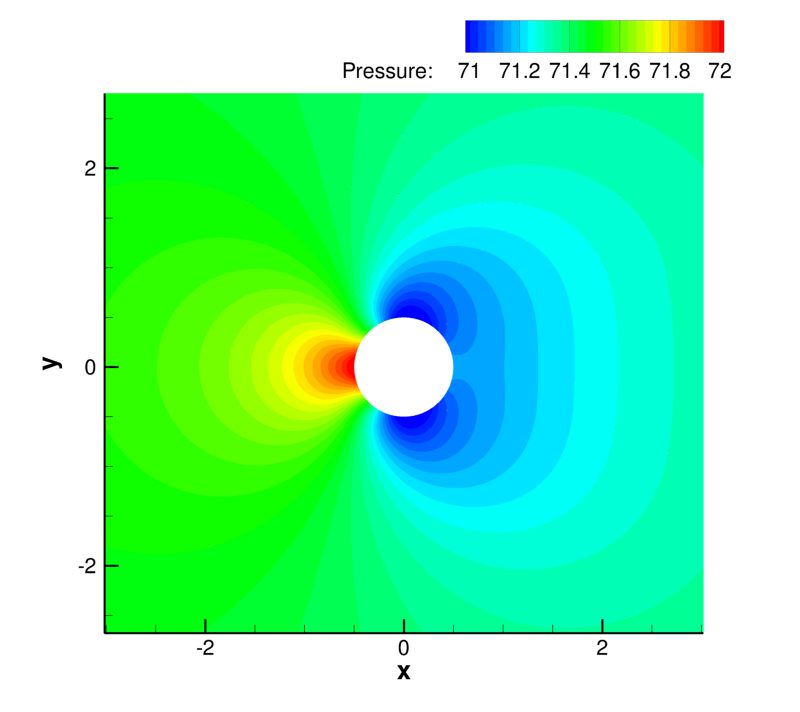
\includegraphics{cylinder_pressure_re20.png}}
    \subfigure[Pressure contours for the $Re = 100$ case.]{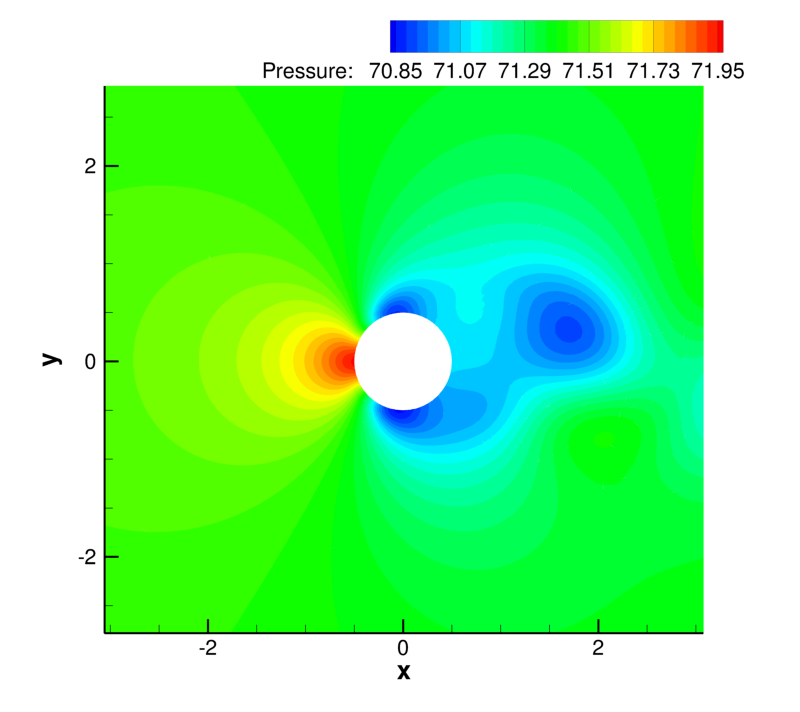
\includegraphics{cylinder_pressure_re100.png}}
  \end{subfigmatrix}
  \caption{Pressure contours for the steady and unsteady (instantaneous) cylinder cases.}
  \label{cylinder_2}
\end{figure}

When the Reynolds number is increased to 100, the flow around the cylinder becomes unsteady and exhibits periodic vortex shedding. This periodic shedding in the wake behind the cylinder can be seen in the instantaneous contours of x-velocity and vorticity in Fig.~\ref{cylinder_3}, and it also results in periodic fluctuations in the force coefficients on the cylinder. HiFiLES reports an average drag coefficient of 1.339 with a maximum deviation from this value of 0.0092, which agree excellently with the values reported by Park et al. of 1.33 and 0.0091 for the average $C_d$ and maximum deviation from it, respectively.  Instantaneous pressure contours for the $Re = 100$ case can be seen in Fig.~\ref{cylinder_2}. The asymmetry that is visible in the pressure contours contributes to the variability in the drag coefficient.

\begin{figure}
  \begin{subfigmatrix}{2}
    \subfigure[X-velocity contours around the circular cylinder for $Re = 100$.]{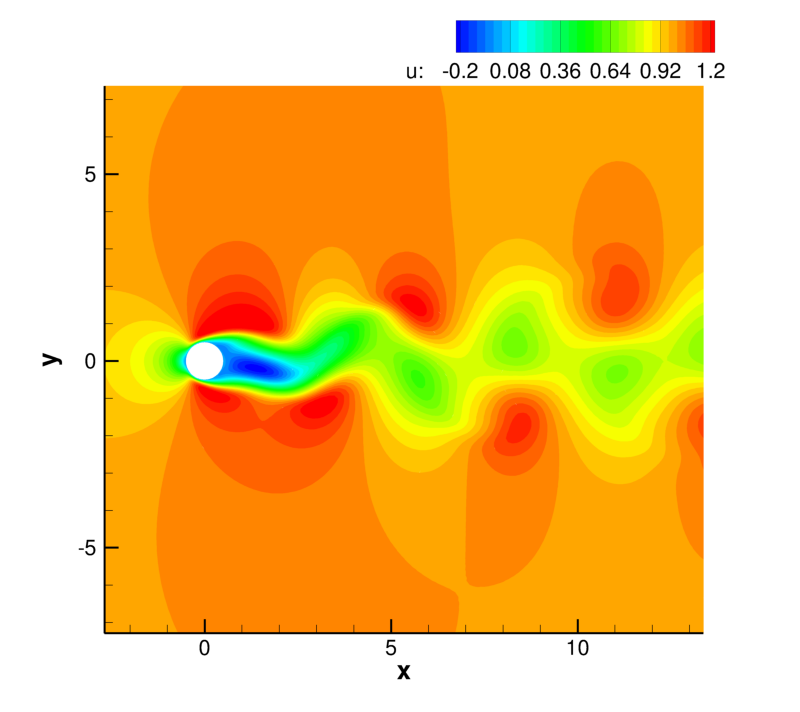
\includegraphics{cylinder_xvelocity_re100.png}}
    \subfigure[Vorticity contours for the $Re = 100$ case.]{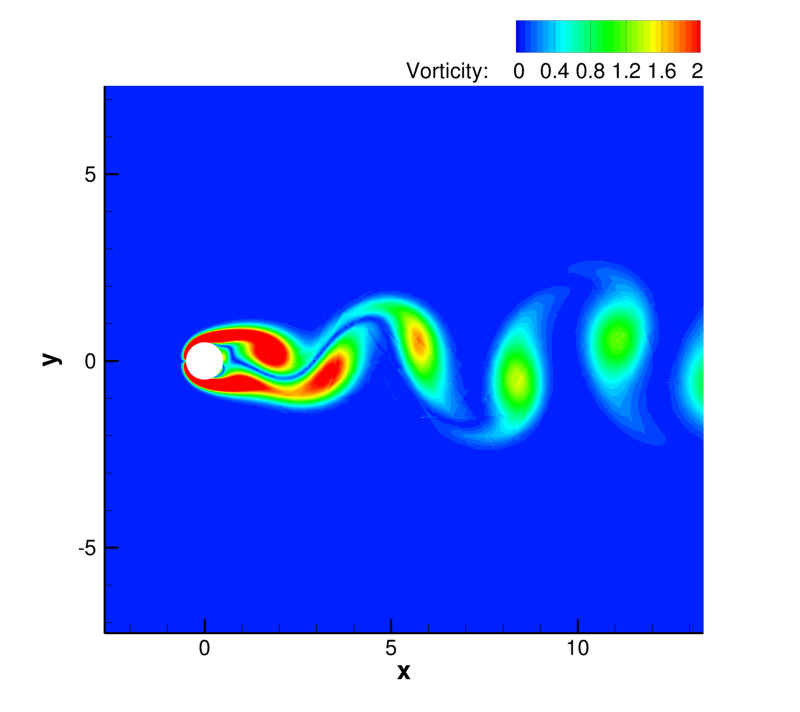
\includegraphics{cylinder_vorticity_re100.png}}
  \end{subfigmatrix}
  \caption{Instantaneous solution contours for the unsteady cylinder case.}
  \label{cylinder_3}
\end{figure}

% SD7003 section
% !TEX root = ./main.tex
\graphicspath{{figures_SD7003/}}% Set graphics path location

\subsection{SD7003 airfoil at 4$\degr$ angle of attack}\label{sd7003airfoil}

Abundant literature documents flow around a SD7003 infinite wing and airfoil. Hence, physical experiments \cite{ol2005comparison,radespiel2007numerical} and numerical simulations \cite{galbraith2008implicit,visbal2009high,castonguay2010simulation,persson2010high,uranga2011implicit} of flow over this geometry can be used to benchmark HiFiLES.

The simulations on the 2D geometry were performed on a circular domain with a radius of $50c$, where $c$ is the airfoil's cord length, centered at the leading edge of the airfoil. The boundary conditions are characteristic on the outer edge and adiabatic no-slip wall on the airfoil. The Mach number for all simulations was $M = 0.2$. The reported lift and drag coefficients in Table \eqref{table:sdAirfoilForce} correspond to the average of lift and drag coefficients over 13 periods after the flow reached a pseudo-periodic state. More details are provided by Williams\cite{williams2013thesis}. 

\begin{table}[htbp]
\centering
\begin{tabular}{ l| l l| l l| l l} 
  
 &  \multicolumn{2}{|c|}{$Re = 10K$}  & \multicolumn{2}{|c|}{$Re = 22K$} & \multicolumn{2}{|c}{$Re = 22K$}  \\ 
 Source & $C_L$ & $C_D$ & $C_L$ & $C_D$ & $C_L$ & $C_D$   \\ 
\hline
 Uranga et al.\cite{uranga2011implicit} & 0.3755 & 0.04978 & 0.6707 & 0.04510 & 0.5730 & 0.02097  \\ 
$c_{dg},\kappa_{dg}$ & 0.3719 & 0.04940 & 0.6722 & 0.04295 & 0.5831 & 0.01975 \\ 
$c_{+},\kappa_{+}$ & 0.3713 & 0.04935 & 0.6655 & 0.04275 & 0.5774 & 0.02005  \\ 
 \end{tabular}
\caption{Time-averaged values of the lift and drag coefficients for the SD7003 airfoil flows with $Re = 10,000, 22,000, 60,000$}
\label{table:sdAirfoilForce} 
 \end{table}

\begin{figure}[htbp]
\centering
\subfigure[Density contours]{
\includegraphics*[trim=0 0 0 0,width=0.48\textwidth]{figure_935a}}
\subfigure[Vorticity contours]{
\includegraphics*[trim=0 0 0 0,width=0.48\textwidth]{figure_935b}}\\

\caption{Density and vorticity contours for the flow with $Re = 10,000$ around the SD7003 airfoil. $p=2$ on unstructured triangular grid with $N = 25,810$ elements}
\label{sdairfoilre10k}
\end{figure}

\begin{figure}[htbp]
\centering
\subfigure[Density contours]{
\includegraphics*[trim=0 0 0 0,width=0.48\textwidth]{figure_936a}}
\subfigure[Vorticity contours]{
\includegraphics*[trim=0 0 0 0,width=0.48\textwidth]{figure_936b}}\\

\caption{Density and vorticity contours for the flow with $Re = 22,000$ around the SD7003 airfoil. $p=2$ on unstructured triangular grid with $N = 25,810$ elements}
\label{sdairfoilre22k}
\end{figure}

\begin{figure}[htbp]
\centering
\subfigure[Density contours]{
\includegraphics*[trim=0 0 0 0,width=0.48\textwidth]{figure_937a}}
\subfigure[Vorticity contours]{
\includegraphics*[trim=0 0 0 0,width=0.48\textwidth]{figure_937b}}\\

\caption{Density and vorticity contours for the flow with $Re = 60,000$ around the SD7003 airfoil. $p=2$ on unstructured triangular grid with $N = 25,810$ elements}
\label{sdairfoilre60k}
\end{figure}

The average lift and drag coefficients are in close agreement with the results by Uranga el. al\cite{uranga2011implicit}. The density contours in Figures \eqref{sdairfoilre10k},\eqref{sdairfoilre22k}, and \eqref{sdairfoilre60k} show that vortical structures are captured for a reasonable distance away from the airfoil despite the fact that elements are coarser away from the airfoil.


\newpage

\subsection{SD7003 wing section at 4$\degr$ angle of attack}
To validate HiFiLES's performance in 3D simulations, we extrude the SD7003 geometry from Section\eqref{sd7003airfoil} by $0.2c$ in the $z$-direction and apply periodic boundary conditions at $z=0$ and $z=0.2c$. Table \eqref{table:sdWingForce} shows the time-averaged lift and drag coefficients.


\begin{table}[htbp]
\centering
\begin{tabular}{ l| l l| l l| l l} 
  
 &  \multicolumn{2}{|c|}{$Re = 10K$}  \\ 
 Source & $C_L$ & $C_D$    \\ 
\hline
 Uranga et al.\cite{uranga2011implicit} & 0.3743 & 0.04967   \\ 
$c_{dg},\kappa_{dg}$ & 0.3466 & 0.04908  \\ 
$c_{+},\kappa_{+}$ & 0.3454 & 0.04903 \\ 
 \end{tabular}
\caption{Time-averaged values of the lift and drag coefficients for the SD7003 wing-section in a flow with $Re = 10,000$}
\label{table:sdWingForce} 
 \end{table}


\begin{figure}[htbp]
\centering
\subfigure[Density contours]{
\includegraphics*[trim=0 0 0 0,width=0.48\textwidth]{figure_939a}}
\subfigure[Vorticity contours]{
\includegraphics*[trim=0 0 0 0,width=0.48\textwidth]{figure_939b}}\\

\caption{Density and vorticity isosurfaces colored by Mach number for the flow with $Re = 10,000$ around the SD7003 wing-section. $p=3$ on unstructured tetrahedral grid with $N = 711,332$ elements}
\label{sdwingre10k}
\end{figure}

It is worth noting that the vortical structures are preserved better than in the 2D case. Table \eqref{table:sdWingForce} demonstrates that HiFiLES provides average lift and drag coefficient estimates in close agreement with experiments.



% Taylor-Green Vortex
% !TEX root = ./main.tex
\graphicspath{{figures_taylorgreen/}}% Set graphics path location

\subsection{Taylor-Green Vortex at Re = 1,600}

The Taylor-Green Vortex (TGV) is a simple test of the resolution of the small scales of a turbulent flow by a numerical method.
The compressible TGV at $Re=1600$ was one of the benchmark problems in the 1st and 2nd International Workshops on High-Order CFD Methods~\cite{wang2013}.
A reference solution was computed by Debonis~\cite{debonis:13} using a high-order dispersion relation-preserving (DRP) scheme on a mesh of $512^3$ elements.
The results presented here were obtained by Bull and Jameson using FR to recover the fourth-order-accurate DG and SD schemes in HiFiLES~\cite{bull2014a,bull2014b}.
We also compare our results to those of Beck and Gassner~\cite{beck:12}, who used a fourth-order filtered DG method on a mesh of $64^3$ elements.
From a simple initial condition in a triply-periodic box of dimensions $[0:2\pi]^3$, interactions between vortices cause the flow to develop in a prescribed manner into a mass of elongated vortices across a range of scales.
The initial condition is specified as
%
\begin{eqnarray}\label{tgv}
u(t_0) &&= u_0 \sin (x/L) \cos (y/L) \cos (z/L), \\
v(t_0) &&= -u_0 \cos (x/L) \sin (y/L) \cos (z/L), \\
w(t_0) &&= 0, \\
p(t_0) &&= p_0 + \frac{\rho_0 V^2_0}{16} \left [ \cos \left (\frac{2x}{L} \right ) + \cos \left (\frac{2y}{L} \right ) \right ] \left [ \cos \left (\frac{2z}{L} \right ) + 2 \right ],
\end{eqnarray}
%
where $L = 1$, $u_0 = 1$, $\rho_0 = 1$ and $p_0 = 100$.
The Mach number is set to 0.08 (consistent with the initial pressure $p_0$) and the initial temperature is 300K.

Figs.~\ref{dissrate} (a) and (b) show the volume-averaged kinetic energy $\langle k \rangle$  on (a) hexahedral meshes of $16^3$, $32^3$ and $64^3$ elements and (b) tetrahedral meshes (formed by splitting the hexahedral meshes in six).
The reference solution, labelled as`DRP-512' is plotted for comparison.
Figs.~\ref{dissrate} (c) and (d) show the kinetic energy dissipation rate, given by $\epsilon = -d \langle k \rangle/dt$ versus the reference solution and the results of Beck and Gassner~\cite{beck:12}, labelled as`Beck-DG-64x4'.
On the finest hexahedral and tetrahedral meshes the kinetic energy and dissipation rate predictions match the reference solution, demonstrating that the high-order numerical scheme is able to resolve the important flow dynamics on a relatively coarse mesh.
As a qualitative measure of the resolution of the turbulent flow structures, Figure \ref{qcrit} shows isosurfaces of the $q$ criterion at four times during the simulation.
The evolution of complex small scale structures is evident.

\begin{figure}[htbp]
\centering
\subfigure[$\langle k \rangle$, hexahedral meshes]{
\includegraphics*[trim=0 0 0 0,width=0.48\textwidth]{tke-SD-hex-mesh}}
\subfigure[$\langle k \rangle$, tetrahedral meshes]{
\includegraphics*[trim=0 0 0 0,width=0.48\textwidth]{tke-SD-tet-mesh.pdf}}\\
\subfigure[$-d \langle k \rangle/dt$, hexahedral meshes]{
\includegraphics*[trim=0 0 0 0,width=0.48\textwidth]{dissrate-SD-hex-mesh.pdf}}
\subfigure[$-d \langle k \rangle/dt$, tetrahedral meshes]{
\includegraphics*[trim=0 0 0 0,width=0.48\textwidth]{dissrate-SD-tet-mesh.pdf}}\\
\caption{\small Taylor-Green vortex results on hexahedral and tetrahedral meshes from Bull and Jameson~\cite{bull2014a}.
(a, b) Evolution of average kinetic energy $\langle k \rangle$; (c, d) dissipation rate $-d \langle k \rangle/dt$.
`SD-$M \times N$' refers to $M^3$ mesh, $N$th-order accurate SD scheme.
(\textbf{- - -}) 4th-order DG on $64^3$ mesh~\cite{beck:12}; ($\circ$) DNS~\cite{debonis:13}.}
\label{dissrate}
\end{figure}

\begin{figure}[htbp]
\centering
\subfigure[$t = 2.5$, $Q=0.5$]{
\includegraphics*[width=0.48\textwidth]{TGV-DG3-hex-64-qcriterion-isosurface-005-velocolor-025s-z-small}}
\subfigure[$t = 5$, $Q=1.5$]{
\includegraphics*[width=0.48\textwidth]{TGV-DG3-hex-64-qcriterion-isosurface-015-velocolor-05s-z-small}}\\
\subfigure[$t = 7.5$, $Q=1.5$]{
\includegraphics*[width=0.48\textwidth]{TGV-DG3-hex-64-qcriterion-isosurface-015-velocolor-075s-z-small}}
\subfigure[$t = 10.75$, $Q=1.5$]{
\includegraphics*[width=0.48\textwidth]{TGV-DG3-hex-64-qcriterion-isosurface-015-velocolor-1075s-z-small}}
\caption{TGV solution on the fine mesh using fourth order accurate DG method, showing isosurfaces of $q$ criterion colored by velocity magnitude at time $t$ = 2.5 to 10.75 seconds.}
\label{qcrit}
\end{figure}



%Square Cylinder
% !TEX root = ./main.tex
\graphicspath{{figures_squarecylinder/}}% Set graphics path location

\subsection{LES of Flow Over a Square Cylinder at Re = 21,400}\label{sqcyl}

Using the FR method to recover the fourth-order accurate SD scheme, the flow over a square cylinder of side $D$ in a domain of $21D \times 12D \times 3.2D$ (see Figure \ref{sqcylmesh}) at $Re = 21,400$ and Mach 0.3 was simulated, for which LDV experimental data is available~\cite{lyn1994,lyn1995}.
A tetrahedral mesh of 87,178 elements was generated giving a total of 1.74M degrees of freedom (D0F) since there are 20 solution points per element at fourth order accuracy.
Time discretization was by the fourth-order five-stage explicit RK scheme.
A total time of 250 seconds was simulated and time-averaged quantities were calculated over the last 100 seconds (approx. 5 flow-through periods).
The WSM model (see Section \ref{lesmodels}) based on the modal Vandermonde filter~\cite{bull2013a} was used with the Breuer-Rodi three-layer wall model~\cite{breuer1994} within 0.2D of the wall.
The computation took around 60 hours on 7 GPUs in the lab's own cluster.
Figure \ref{sqcylmesh} shows the computational mesh including all the DoF.
Figure \ref{sqcylqcrit} shows an isosurface of the $q$-criterion colored by velocity magnitude, illustrating the structures present in the turbulent boundary layer and wake.
Figures \ref{sqcylplots} (a, b) show the normalized mean streamwise and vertical velocity components $\langle u \rangle/u_B$ and $\langle v \rangle/u_B$ respectively along several vertical lines in the wake.
Figures \ref{sqcylplots} (c, d) show the normalized mean Reynolds stress components $\langle u'u' \rangle/u_B^2$ and $\langle u'v' \rangle/u_B^2$ along the same lines.
For comparison, high-order LES results computed by by Lodato and Jameson~\cite{lodato2012b} using the SD method and the WSM model on a hexahedral mesh of 2.3M DoF are plotted.
Mean velocities are accurately predicted although the accuracy is reduced near the cylinder owing to the coarse tetrahedral resolution in the boundary layer.
The Reynolds stresses are less accurately predicted than the mean velocities but are broadly correct.
These results highlight the advantages of using HiFiLES for LES of turbulent flows: the ability to obtain good results on coarse meshes and the ability to use unstructured tetrahedral meshes.


\begin{figure}[h] \tt
\centering
\subfigure[geometry]{
\includegraphics*[width=0.61\textwidth]{sqcyl-geom-small}}
\subfigure[boundary layer mesh]{
\includegraphics*[width=0.35\textwidth]{sqcyl-tet-coarse3-blmesh}}
\caption{Square cylinder geometry and tetrahedral boundary layer mesh showing all degrees of freedom}
\label{sqcylmesh}
\end{figure}

\begin{figure}[h] \tt
\centering
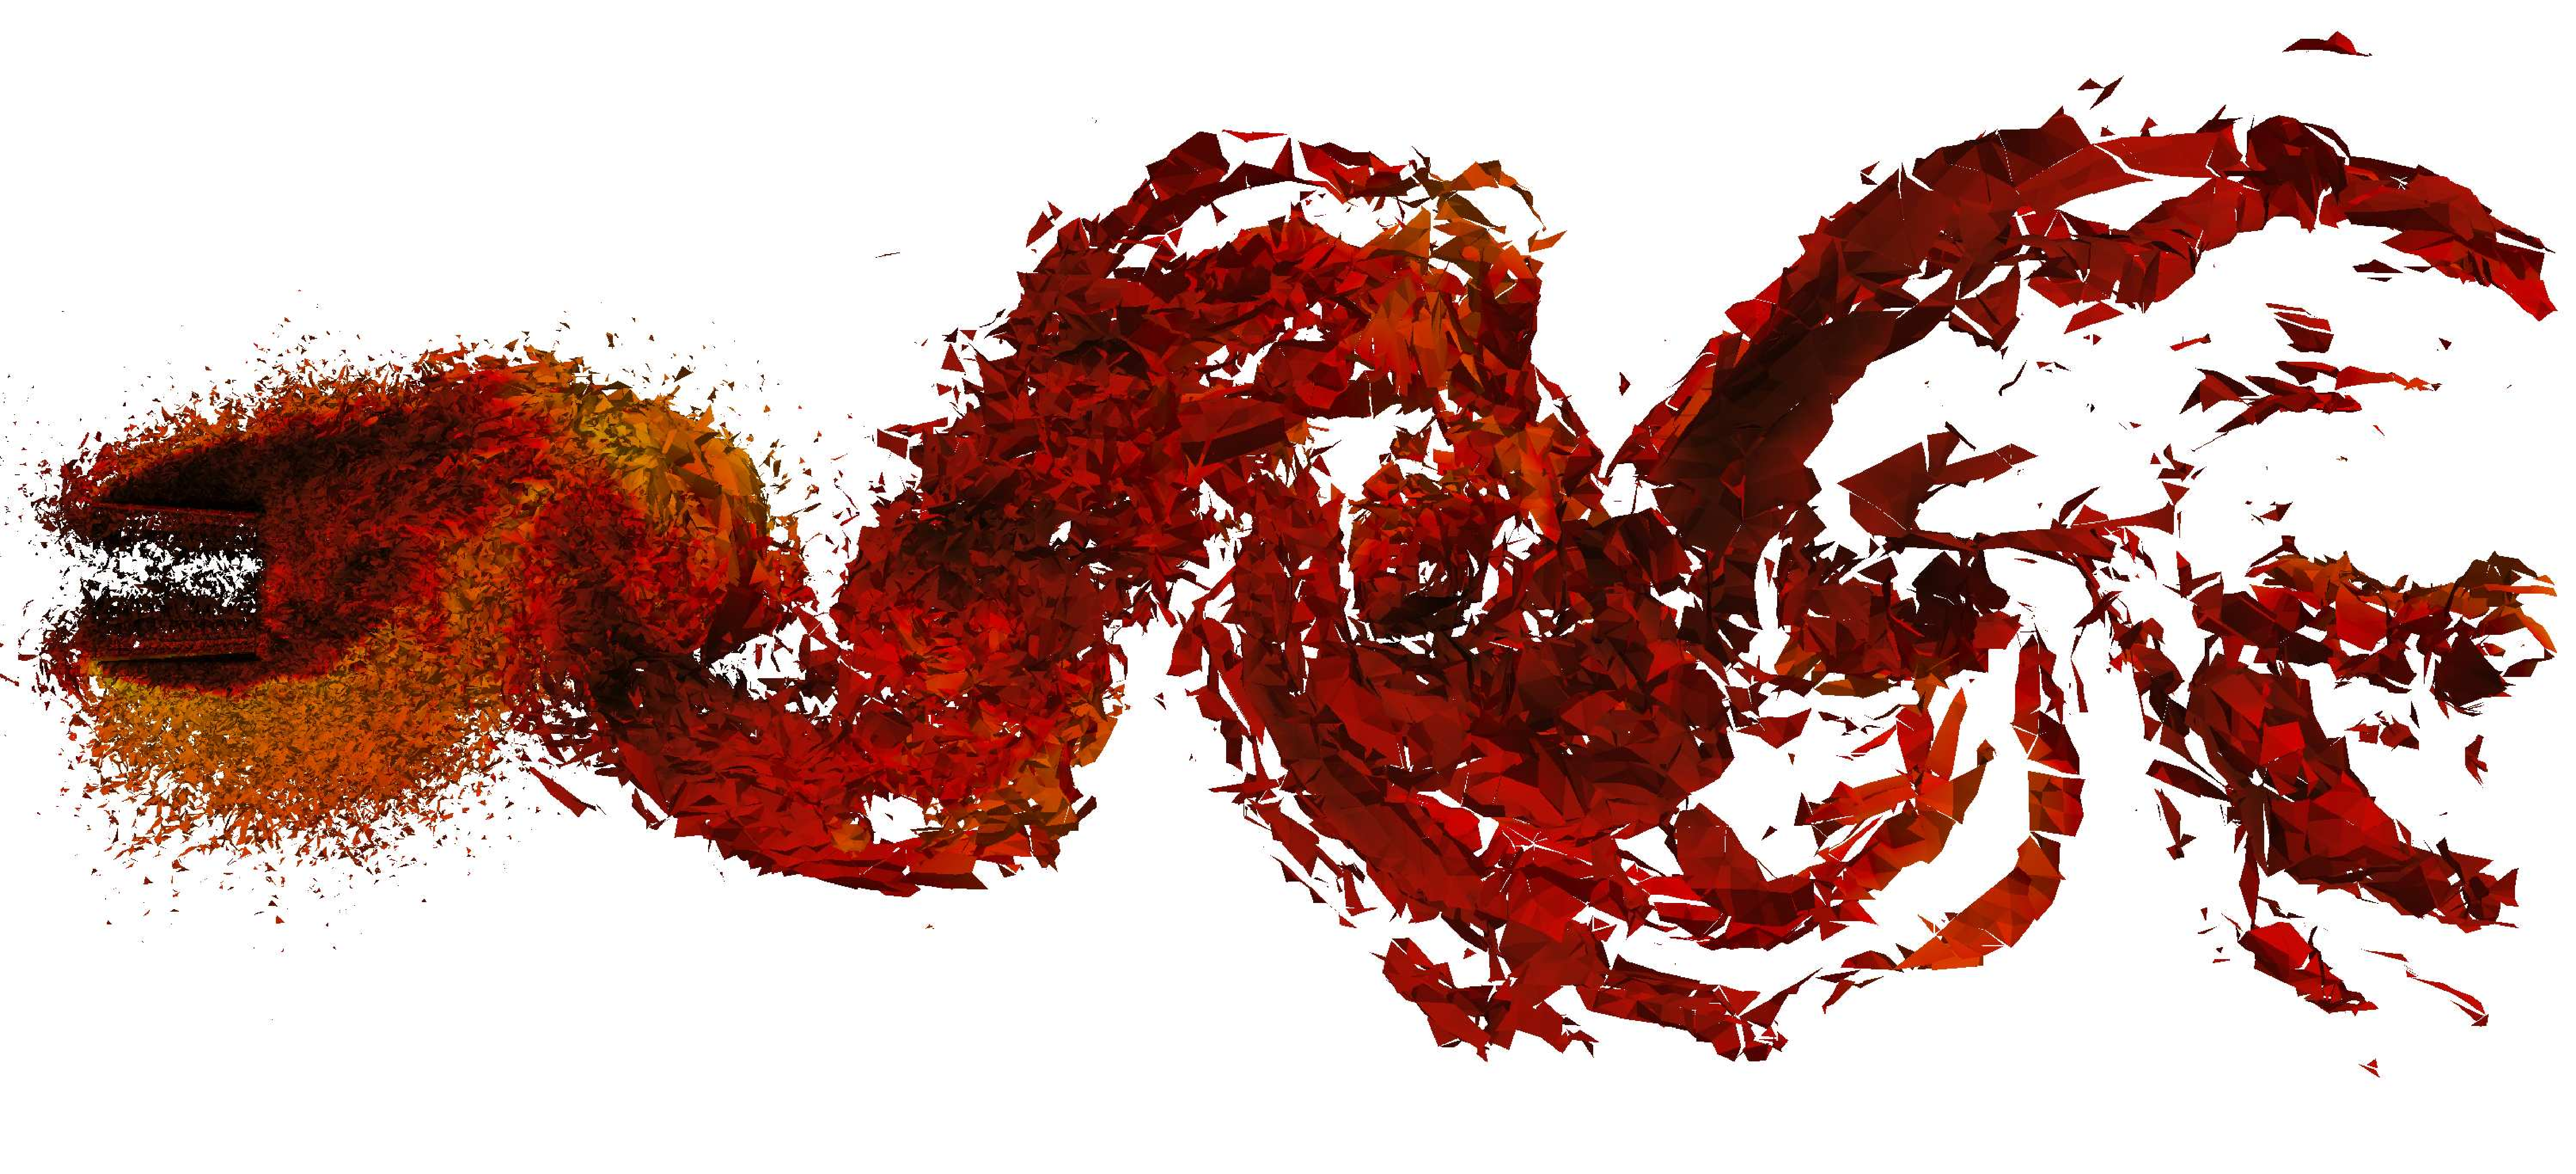
\includegraphics[width=0.9\textwidth]{sqcyl-tet-wsm-newwallfn-coarse3-qcrit-010-velomag.pdf}
\caption{Isosurface of the $q$-criterion colored by velocity magnitude showing the wake behind the square cylinder}
\label{sqcylqcrit}
\end{figure}

\begin{figure}[h]
\centering
\subfigure[Mean streamwise velocity $\langle u \rangle/u_B$]{
\includegraphics*[width=0.8\textwidth]{sqcyl-tet-wsm-newfilt-coarse-fixbc-meanu-vprofile-small.pdf}}\\
\subfigure[Mean vertical velocity $\langle v \rangle/u_B$]{
\includegraphics*[width=0.8\textwidth]{sqcyl-tet-wsm-newfilt-coarse-fixbc-meanv-vprofile-small.pdf}}\\
\subfigure[Mean Reynolds stress $\langle u'u' \rangle/u_B^2$]{
\includegraphics*[width=0.8\textwidth]{sqcyl-tet-wsm-newfilt-coarse-fixbc-meanuu-vprofile-small.pdf}}\\
\subfigure[Mean Reynolds stress $\langle u'v' \rangle/u_B^2$]{
\includegraphics*[width=0.8\textwidth]{sqcyl-tet-wsm-newfilt-coarse-fixbc-meanuv-vprofile-small.pdf}}
\caption{\small (a) Mean streamwise and vertical velocity and mean Reynolds stresses along vertical lines in the wake.
(---) current results, (- - - ) 4th order SD+WSM on hexahedral mesh by Lodato and Jameson~\cite{lodato2012b}, ($\circ$) LDV experiments by Lyn et al.~\cite{lyn1994,lyn1995}.}
\label{sqcylplots}
\end{figure}



%NACA 0012 airfoil
% !TEX root = ./main.tex
\graphicspath{{figures_RANS_naca0012/}}% Set graphics path location

\subsection{NACA 0012 airfoil at 0$\degr$ angle of attack, Re = 6 million, Ma = 0.15}
In this section, the NACA 0012 airfoil is used to study the accuracy of the SA turbulence model coupled with FR. The NACA 0012 is commonly used as a validation case for all turbulence models and a large database of results are available at the NASA Turbulence Modeling Resource website. A 6,539 element quad/triangle mixed mesh is used with a NACA 0012 airfoil of chord length 1.0 and a farfield boundary 20 chord lengths away. The results are compared with CFL3D and experimental results from Gregory \& O'Reilly, NASA R\&M 3726, Jan 1970.

\begin{figure}
  \begin{subfigmatrix}{2}
    \subfigure[Zoomed view of the mixed element mesh near the NACA 0012 airfoil.]{\includegraphics{NACA0012_Re6mil_mesh.eps}}
    \subfigure[X-momentum contours near the NACA 0012 airfoil]{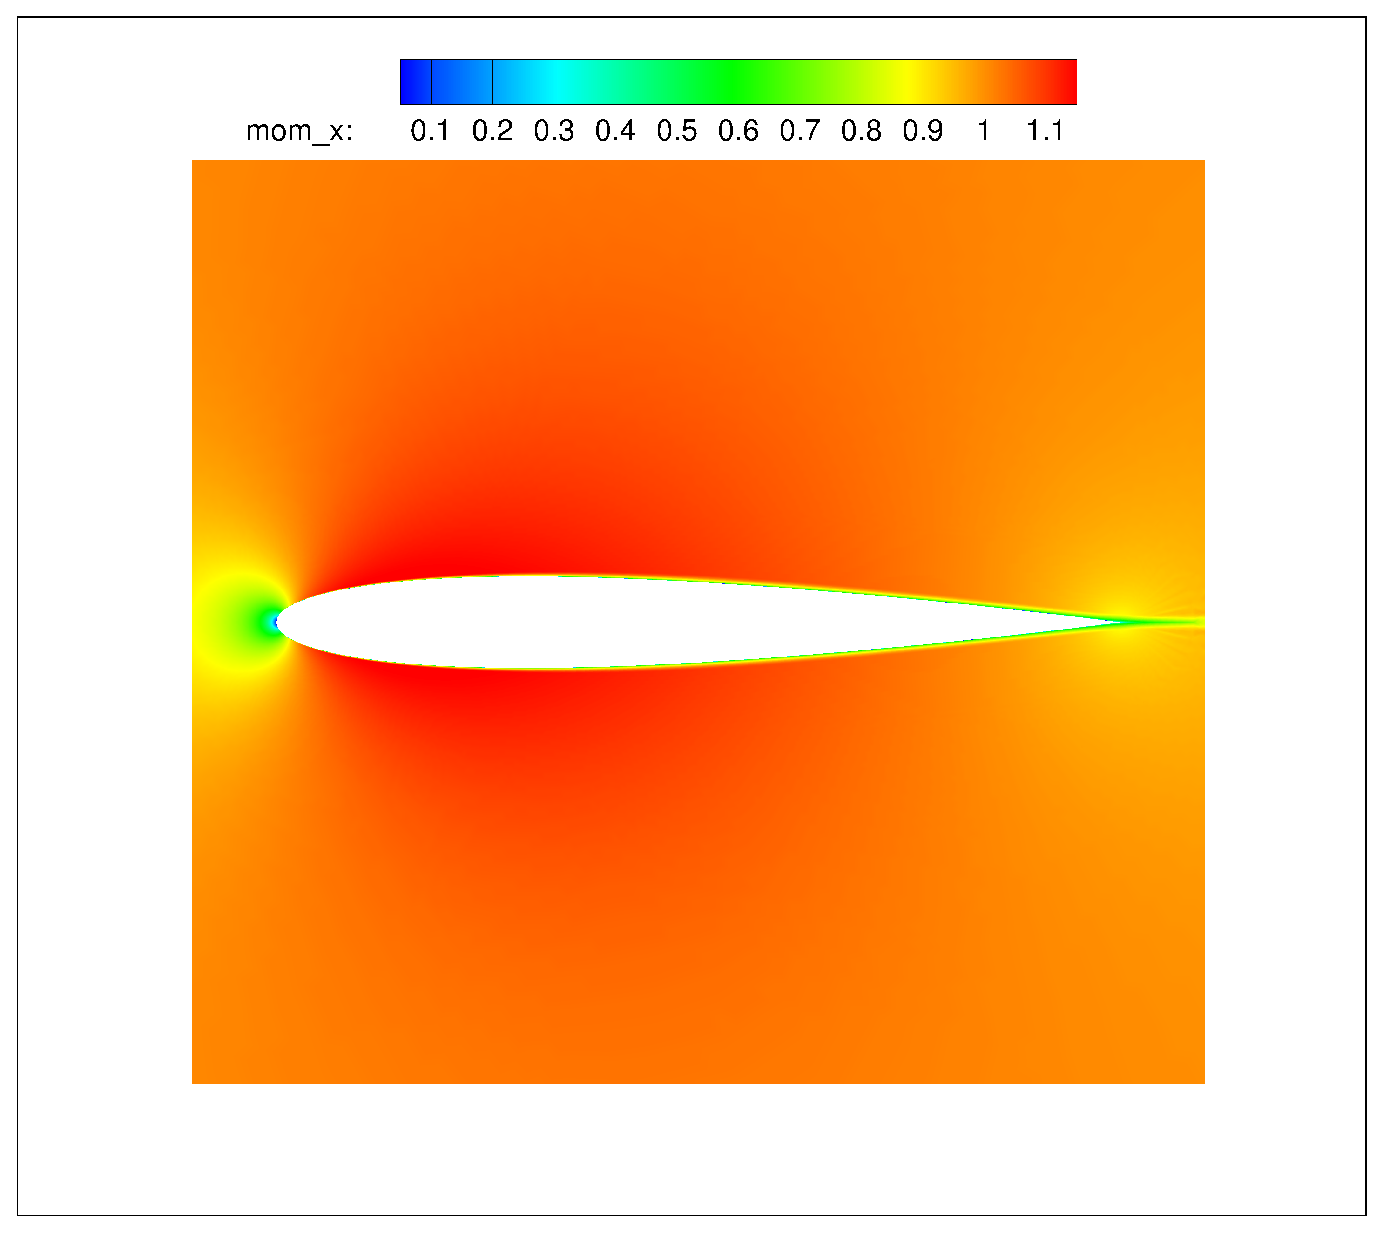
\includegraphics{NACA0012_Re6mil_alp0_momx.eps}}
  \end{subfigmatrix}
  \caption{Turbulent flow past a NACA 0012 airfoil at Re = 6 million, Ma = 0.15, $\alpha = 0^{\circ}$ using FR to recover 4th order accurate DG method and the SA turbulence model.}
  \label{RANS_naca0012}
\end{figure}

\begin{figure}
\centering
  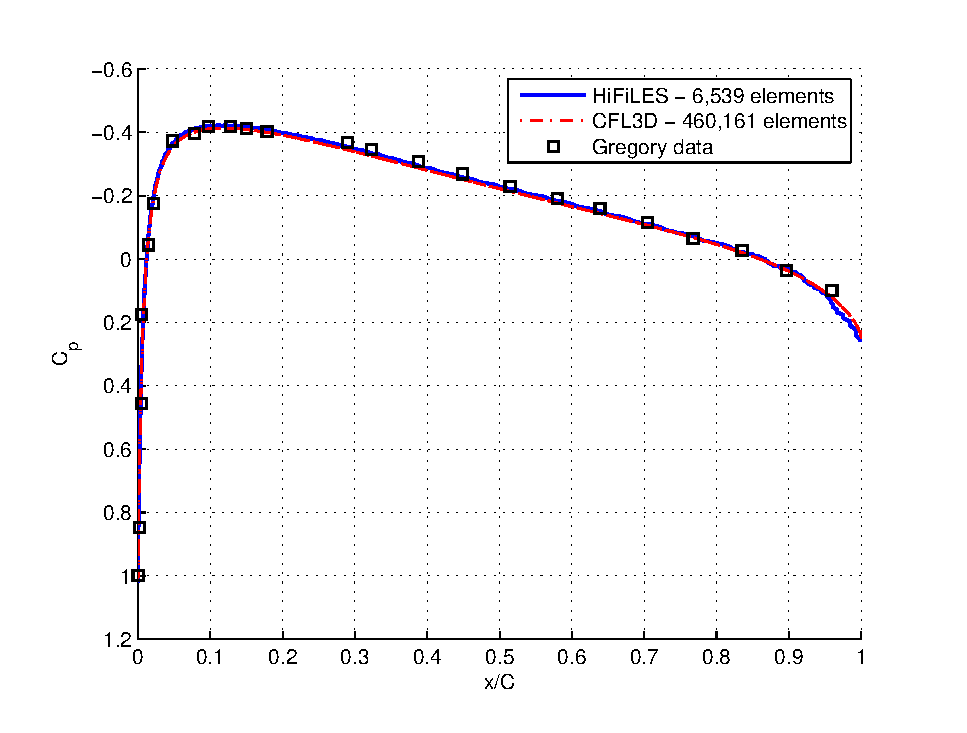
\includegraphics[width=0.48\textwidth]{cp.eps}
  \caption{Pressure coefficient on the NACA 0012 airfoil at Re = 6 million, Ma = 0.15, $\alpha = 0^{\circ}$ using FR to recover 4th order accurate DG method and the SA turbulence model.}
  \label{RANS_naca0012_cp}
\end{figure}


% Other verification tests in time? Efficiency/scalability studies?



%% !TEX root = ./main.tex



% Add additional cases by creating a "case_name.tex" file with a corresponding "figures_name" directory to hold all of your figures for that case. This will help keep organized and avoid conflicts. Lastly, simply add an include statement lie those above for your new case. Don't forget to "git add" and commit/push your changes up to the master.

% !TEX root = ./main.tex

\section{Conclusion}
\label{sec:conclusion}

In this work, we have presented a comprehensive description, verification and validation of the HiFiLES solver. In its first release, HiFiLES offers to its users an optimal implementation of the Flux Reconstruction methodology in unstructured 3D grids using GPUs or traditional MPI. The code has been tested in some difficult Navier-Stokes and Large Eddy Simulation problems with very satisfactory results.

Despite considerable advances in the accuracy and versatility of subgrid-scale models, current industrial CFD codes are restricted in their ability to perform LES of turbulent flows by the use of highly dissipative second-order numerical schemes.
Therefore, in order to advance the state of the art in industrial CFD, it is necessary to move to high-order accurate numerical methods.
The ESFR family of schemes are ideal for resolving turbulent flows due to low numerical dissipation and high-order accurate representation of solution gradients at the small scales.
Advanced subgrid-scale models have been implemented in HiFiLES for all element types, enabling simulation of turbulent flows over complex geometry.
The development of the first high-order accurate solver for unstructured meshes incorporating LES modeling capabilities represents a significant step towards tackling challenging compressible turbulent flow problems of practical interest.
Future work will include the development of dynamic modeling, non-equilibrium wall modeling and other advanced modeling concepts in order to improve predictions of complex flows on coarse meshes.

% !TEX root = ./main.tex

\section*{Acknowledgements}

The authors would like to acknowledge the support for this work provided by the Stanford Graduate Fellowships, National Science Foundation Graduate Fellowships, the National Science Foundation under Grant 1114816, and the Air Force Office of Scientific Research under Grant FA9550--10--1--0418.

\bibliographystyle{aiaa}

\bibliography{references}

 \end{document}


